\chapter{Computing a best choice recommendation}
\label{sec:4}

\abstract*{ In this chapter we present the \Rubis best choice recommender system. To illustrate the approach we use a best office site selection problem. We show how to explore the given performance tableau and compute the corresponding outranking digraph. We present the pragmatic principles that govern our best choice recommendation algorithm and solve the illustrative best office site choice problem.}

\begin{quotation}
  ``... The goal of our research was to design a resolution method ... that is easy to put into practice, that requires as few and reliable hypotheses as possible, and that meets the needs [of the decision maker]...''

  --\citep*{ROY-1966}\index{Roy@\textsl{B. Roy}}.
\end{quotation}
\vspace{1cm}

\abstract{ In this chapter we present the \Rubis best choice recommender system. We illustrate our \Rubis approach with a best office site selection problem. We show how to explore the given performance tableau and compute the corresponding outranking digraph. We present the pragmatic principles that govern our best choice recommendation algorithm and solve the illustrative best office site choice problem.}

\section{What office site to choose?}
\label{sec:4.1}

A SME, specialized in printing and copy services, has to move into new offices, and its CEO has gathered seven \emph{potential new office sites} (see Table~\vref{tab:4.1}).
\begin{table}[h]
\caption{The potential new office sites}
\label{tab:4.1}       % Give a unique label
\begin{center}
  %\begin{small}
    \begin{tabular}{c|l|l|l}
      \svhline\noalign{\smallskip}
      ID & Name & Address & Comment\\
      \noalign{\smallskip}\hline\noalign{\smallskip}
    A &   Ave  &  Avenue de la liberté &  High standing city center\\
    B &   Bon  &  Bonnevoie &             Industrial environment\\
    C &   Ces  &  Cessange &              Residential suburb location\\
    D &   Dom  &  Dommeldange &           Industrial suburb environment\\
    E &   Bel  &  Esch-Belval &           New and ambitious urbanization far from the city\\
    F &   Fen  &  Fentange &              Out in the countryside\\
      G &   Gar  &  Avenue de la Gare &     Main city shopping street\\
      \noalign{\smallskip}\hline
    \end{tabular}
  %\end{small}
\end{center}
\end{table}

Three \emph{decision objectives}, in order of decreasing importance, are guiding the CEO's choice:
\begin{enumerate}[leftmargin=1cm]
\item \emph{maximize} the future turnover of the SME,
\item \emph{minimize} the future yearly costs induced by the moving,
\item \emph{maximize} the new working conditions.
\end{enumerate}

The decision consequences to take into account for evaluating the potential new office sites with respect to each of the three objectives are modelled by the \emph{family of performance criteria} \footnote{See \citealp{ROY-2000}} shown in Table~\vref{tab:4.2}.
\begin{table}[h]
\caption{The family of performance criteria}
\label{tab:4.2}       % Give a unique label
\begin{center}
    \begin{tabular}{l|c|c|c|l}
      \svhline\noalign{\smallskip}
      Objective & ID & Name & Weight & Comment\\
      \noalign{\smallskip}\hline\noalign{\smallskip}
    Yearly costs  &       C &   Costs &  45 &     Annual rent, charges, and cleaning\\
    \             &  \      & \        &  \ & \ \\
    Future turnover   &   Pr  & Proximity  & 32 & Distance from town center\\
    Future turnover   &   V  &  Visibility & 26 & Circulation of potential customers \\
    Future turnover   &   St &   Standing & 23 &   Image and presentation\\
    \                 &   \   & \          &  \ & \  \\
    Working conditions &  W  &  Space   &   10 &  Working space\\
    Working conditions &  Cf &  Comfort  &  6 &  Quality of office equipment\\
    Working conditions &  P  &  Parking  &  3 &  Available parking facilities\\
      \noalign{\smallskip}\hline
    \end{tabular}   
  \end{center}
\end{table}

In Table~\vref{tab:4.2} we notice that the \emph{Costs} criterion admits the highest significance ($45$), followed by the \emph{Future turnover} criteria $(32 + 26 + 23 = 81)$, The \emph{Working conditions} criteria are the less significant $(10 + 6 + 3 = 19)$ \footnote{These criteria weights were supposedly established with a swing weighing MCDA method \citep{KEE-1976}.}. It follows that the CEO considers \emph{maximizing the future turnover} the most important objective ($81.0$), followed by minizing the future yearly costs ($45.0$), and less important, \emph{maximizing working conditions} ($19.0$). 

The evaluation of the seven potential new sites on each performance criterion are gathered in a \emph{performance table} shown in Table~\vref{tab:4.3}.
\begin{table}[h]
\caption{Performance evaluations of the potential office sites}
\label{tab:4.3}       % Give a unique label
\begin{center}
    \begin{tabular}{l|c|c|c|c|c|c|c}
      \svhline\noalign{\smallskip}
    Criterion  &    A  &      B &       C &       D &       E &        F &        G\\
       \noalign{\smallskip}\hline\noalign{\smallskip}

    Costs      &   35.0K€ &  17.8K€  & 6.7K€  &  14.1K€ &  34.8K€ &  18.6K€ &  12.0K€\\
    \          &   \      &  \     &   \     &   \    &    \    &    \    &    \ \\
    Proximity     &   100    &  20 &      80    &   70    &   40    &   0    &    60 \\
    Visibility     &   60     &  80  &     70    &   50    &   60    &   0    &    100 \\
    Standing      &   100   &   10   &    0     &   30    &   90    &   70   &    20 \\
    \           &   \     &   \    &    \     &   \     &   \     &   \    &    \  \\
    Working space      &   75    &   30   &    0     &   55    &   100   &   0    &    50  \\
    Working comfort      &   0     &   100  &    10    &   30    &   60    &   80   &    50 \\
    Parking     &   90    &   30   &    100   &   90    &   70    &   0    &    80 \\
      \noalign{\smallskip}\hline
    \end{tabular}
  \end{center}
\end{table}

All criteria, except the \emph{Costs} Criterion, admit for grading a qualitative satisfaction scale from $0\%$ (worst) to $100\%$ (best). We may thus notice in Table~\vref{tab:4.3} that site \texttt{A} (\emph{Ave}) is the most expensive, but also $100\%$ satisfying the \emph{Proximity} as well as the  \emph{Standing} criterion. Whereas site \texttt{C} (\emph{Ces}) is the cheapest one; providing however no satisfaction at all on both the \emph{Standing} and the \emph{Working Space} criteria.

Concerning yearly costs, we suppose that the CEO is indifferent up to a performance difference of $1000.00$€, and he actually prefers a site when there is at least a positive difference of $2500.00$€. The grades observed on the six qualitative criteria (measured in percentages of satisfaction) are very subjective and rather imprecise. The CEO is hence \emph{indifferent} up to a satisfaction difference of $10\%$, and he claims a significant \emph{preference} when the satisfaction difference is at least of $20\%$.  Furthermore, a satisfaction difference of $80\%$ represents for him a \emph{considerably large} performance difference, triggering the case given a \emph{polarisation} of the preferential situations \citep{BIS-2013}. 

In view of Table~\vref{tab:4.3}, what is now the office site we may recommend to the CEO as \textbf{best choice}?

\section{The given performance tableau}
\label{sec:4.2}


In file \texttt{officeChoice.py}, stored in the \texttt{examples} directory of the \Digraph resources, a corresponding, \texttt{PerformanceTableau}\index{PerformanceTableau@\texttt{PerformanceTableau} class} object, is provided. We may inspect its actual content with the computing resources provided by the \texttt{perfTabs} module \index{perfTabs@\texttt{perfTabs} module}.
\begin{lstlisting}[caption={Inspecting the \texttt{officeChoice} performance tableau.},label=list:4.1]
>>> from perfTabs import PerformanceTableau
>>> t = PerformanceTableau('officeChoice')
>>> t
 *------- PerformanceTableau instance description ------*
   Instance class     : PerformanceTableau
   Instance name      : officeChoice
   Actions            : 7
   Objectives         : 3
   Criteria           : 7
   NaN proportion (%) : 0.0
   Attributes         : ['name', 'actions', 'objectives',
                         'criteria', 'weightPreorder',
			 'NA', 'evaluation']
>>> t.showPerformanceTableau()
 *----  performance tableau -----*
  Criteria|  'C'        'Cf'   'P'   'Pr'   'St'   'V'    'W'   
  Weights |  45.00      6.00   3.00  32.00  23.00  26.00  10.00    
  --------|----------------------------------------------------
   'Ave'  | -35000.00   0.00  90.00 100.00 100.00  60.00  75.00  
   'Bon'  | -17800.00 100.00  30.00  20.00  10.00  80.00  30.00  
   'Ces'  |  -6700.00  10.00 100.00  80.00   0.00  70.00   0.00  
   'Dom'  | -14100.00  30.00  90.00  70.00  30.00  50.00  55.00  
   'Bel'  | -34800.00  60.00  70.00  40.00  90.00  60.00 100.00  
   'Fen'  | -18600.00  80.00   0.00   0.00  70.00   0.00   0.00  
   'Gar'  | -12000.00  50.00  80.00  60.00  20.00 100.00  50.00  
\end{lstlisting}

We thus recover all the input data shown in Section~\vref{sec:4.1}. Notice the \emph{negative} figures on the Costs criterion indicate a negative preference direction: the \emph{lower} the costs, the \emph{better} it is. We may use the \texttt{showCriteria()}\index{showCriteria@\texttt{showCriteria()}} method for measuring the actual preference discrimination we observe on each criterion.
\begin{lstlisting}[caption={Inspecting the performance criteria.},label=list:4.2]
>>> t.showCriteria(IntegerWeights=True)
 *----  criteria -----*
  C 'Costs'
   Scale = (Decimal('0.00'), Decimal('50000.00'))
   Weight = 45
   Threshold ind : 1000.00 + 0.00x ;  percentile:  9.5
   Threshold pref : 2500.00 + 0.00x ; percentile: 14.3
  Cf 'Comfort'
   Scale = (Decimal('0.00'), Decimal('100.00'))
   Weight = 6
   Threshold ind : 10.00 + 0.00x ;  percentile:   9.5
   Threshold pref : 20.00 + 0.00x ; percentile:  28.6
   Threshold veto : 80.00 + 0.00x ; percentile:  90.5
    ...
\end{lstlisting}
On the \emph{Costs} criterion, $9.5\%$ of the performance differences are considered insignificant and $14.3\%$ below the preference discrimination threshold (see Listing~\vref{list:4.2} lines 6-7). On the qualitative \emph{Comfort} criterion, we observe again $9.5\%$ of insignificant performance differences (line 11). Due to the imprecision in the subjective grading, we notice here $28.6\%$ of performance differences below the preference discrimination threshold (Line 12). Furthermore, $100.0 - 90.5 = 9.5\%$ of the performance differences are judged \emph{considerably large} (Line 13) and triggering hence a polarisation of the concerned outranking situations \citep{BIS-2013}. Same information is available for all the other criteria. 
 
A colorful comparison of all the performances is shown in Figure~\vref{fig:4.1} by the \emph{heatmap}\index{showHTMLPerformanceHeatmap@\texttt{showHTMLPerformanceHeatmap()}} statistics, illustrating the respective quantile class of each performance. As the set of potential alternatives is tiny, we choose here a classification into performance quintiles.
\begin{lstlisting}
>>> t.showHTMLPerformanceHeatmap(colorLevels=5,\
...                              rankingRule=None)
\end{lstlisting}
    \begin{figure}[h]
%\sidecaption
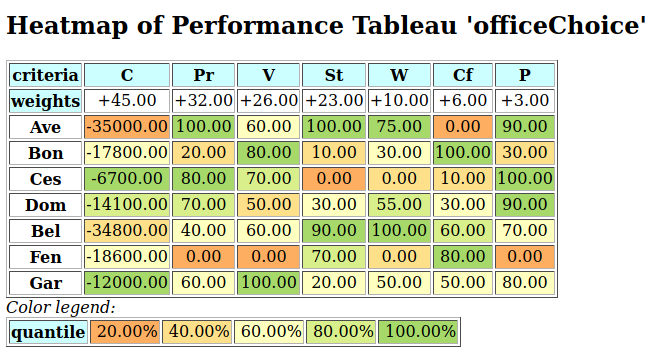
\includegraphics[width=11cm]{Figures/4-1-officeChoiceHeatmap.png}
\caption{Unranked heatmap of the office choice performance tableau}
\label{fig:4.1}       % Give a unique label
\end{figure}

Site \texttt{A} (\emph{Ave}) shows extreme and contradictory performances: highest \emph{Costs} and no \emph{Working Comfort} on the one hand, and total satisfaction with respect to \emph{Standing}, \emph{Proximity} and \emph{Parking facilities} on the other hand. Similar, but opposite, situation is given for site \texttt{C} (\emph{Ces}): unsatisfactory \emph{Working Space}, no \emph{Standing} and no \emph{Working Comfort} on the one hand, and lowest \emph{Costs}, best \emph{Proximity} and \emph{Parking facilities} on the other hand. Contrary to these contradictory alternatives, we observe two appealing compromise decision alternatives: sites \texttt{D} (\emph{Dom}) and \texttt{G} (\emph{Gar}). Finally, site \texttt{F} (\emph{Fen}) is clearly the less satisfactory alternative of all.

To help now the CEO choosing the best office site, we are going to compute pairwise outranking situations on the set of potential decision alternatives (see \citet{BIS-2013}).

\section{Computing the outranking digraph}
\label{sec:4.2}

\begin{definition}[Outranking situation]\label{def:outranking}\index{outranking!situation}

\noindent For two potential decision alternatives $x$ and $y$:
\begin{itemize}[leftmargin=0.5cm,rightmargin=0.5cm]
\item ``Alternative $x$ \emph{outranks} alternative $y$'', denoted $(x \succsim y)$, is given when there is:
   \begin{enumerate}
     \item A \emph{majority} of criteria significance concordantly supporting that alternative $x$ is \emph{at least as well performing as} alternative $y$, and
     \item \emph{No considerable} counter-performance observed on any discordant criterion.      
    \end{enumerate}
\item ``Alternative $x$ \emph{does not outrank} $y$'', denoted $(x \not\succsim y)$, is given when there is:
   \begin{enumerate}
    \item A \emph{majority} of criteria concordantly supporting that alternative $x$ is \textbf{not} \emph{at least as well performing as} alternative $y$, and
    \item \emph{No considerable} better performance observed on any discordant criterion. 
    \end{enumerate}
\item Otherwise, the outranking situation between alternatives $x$ and $y$ is considered to be \emph{indeterminate}.
\end{itemize}
\end{definition}
The credibility of each pairwise outranking situation, denoted $r(x \succsim y)$, is measured in a bipolar significance valuation $[-1.0, 1.0]$, where \emph{positive} terms $r(x \succsim y)\, >\, 0.0$ indicate a \emph{validated}, and \emph{negative} terms $r(x \succsim y)\, <\, 0.0$ indicate a \emph{non-validated} outranking situation. The \emph{median} value $r(x \succsim y)\, = \,0.0$ represents an \emph{indeterminate} situation (see \citet{BIS-2004a} and \citet{BIS-2013}).   

For computing such a bipolar-valued binary outranking relation from the given performance tableau $t$, we use the \texttt{BipolarOutrankingDigraph}\index{BipolarOutrankingDigraph} constructor from the \texttt{outrankingDigraphs}\index{outrankingDigraphs} module. The corresponding
\texttt{showHTMLRe\-lationTable}\index{showHTMLRelationTable} method shows here the resulting bipolar-valued adjacency matrix in a system browser window (see Fig.~\vref{fig:4.2}).
\begin{lstlisting}[caption={Computing a bipolar-valued outranking digraph},label=list:4.3]
>>> from outrankingDigraphs import BipolarOutrankingDigraph
>>> g = BipolarOutrankingDigraph(t)
>>> g.showHTMLRelationTable()
\end{lstlisting}
\begin{figure}[h]
\sidecaption[t]
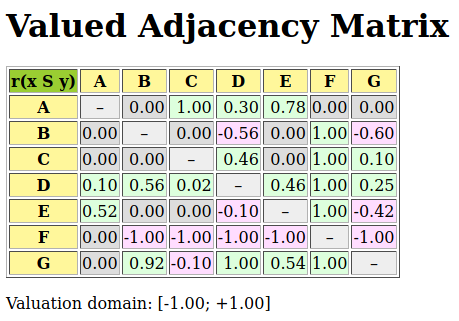
\includegraphics[width=7cm]{Figures/4-2-officeChoiceOutranking.png}
\caption{Bipolar-valued adjacency matrix. In the resulting outranking relation we may notice, on the one hand, that Alternative \texttt{D} is \emph{positively outranking} all other potential office sites. On the other hand, alternatives \texttt{A} (the most expensive) and \texttt{C} (the cheapest) are \emph{not outranked} by any other site}
\label{fig:4.2}       % Give a unique label
\end{figure}
Alternative \texttt{D} gives a \Condorcet winner\footnote{See Chapter~\vref{sec:7} on computing the winner of an election.}, whereas alternatives \texttt{A} (the most expensive) and \texttt{C} (the cheapest) give in fact \emph{weak} \Condorcet winners.\index{computeCondorcetWinners@\texttt{computeCondorcetWinners()}}\index{computeWeakCondorcetWinners@\texttt{computeWeakCondorcetWinners()}}
\begin{lstlisting}
>>> g.computeCondorcetWinners()
 ['D']
>>> g.computeWeakCondorcetWinners()
 ['A', 'C', 'D']
\end{lstlisting}

From theory, we know that outranking digraphs are \emph{weakly complete}\index{weakly complete}, i.e. for all $x$ and $y$ in $X$, $r(x \succsim y)\, <\, 0.0$ implies that $r(y \succsim x)\, \geq\, 0.0$. And, they verify the \emph{coduality principle}\index{coduality principle}:  $r(x \not\succsim y) \;=\; r(y \succnsim x)$ \citep{BIS-2013}.

\begin{definition}[Strict outranking situation]\label{def:strictOutranking}\index{outranking!strict situation}

\noindent For two potential decision alternatives $x$ and $y$:
\begin{itemize}[leftmargin=0.5cm,rightmargin=0.5cm]
\item ``Alternative $x$ \emph{stricly outranks} alternative $y$'', denoted $(x \succnsim y)$, is given when there is:
   \begin{enumerate}
     \item A \emph{majority} of criteria significance concordantly supporting that alternative $x$ is \emph{better performing than} alternative $y$, and
     \item \emph{No considerable} counter-performance observed on any discordant criterion.      
    \end{enumerate}
\item ``Alternative $x$ \emph{is not strictly outranking} alternative $y$'', denoted $(x \not\succnsim y)$, is given when there is:
   \begin{enumerate}
    \item A \emph{majority} of criteria concordantly supporting that alternative $x$ is \emph{not better performing than} alternative $y$, and
    \item \emph{No considerable} better performance observed on any discordant criterion. 
    \end{enumerate}
\item Otherwise, the \emph{strict} outranking situation between alternatives $x$ and $y$ is considered to be \emph{indeterminate}.
\end{itemize}
\end{definition}

Our best office site choice will now be based on such strict outranking situations.

\section{Designing a best choice recommender system}
\label{sec:4.3}

Traditionally, solving a best-choice problem consists in finding \emph{the} unique best decision alternative. We adopt here instead a modern recommender system’s approach which shows a non empty subset of decision alternatives which contains by construction the potential best alternative(s).

Our five \emph{pragmatic principles} for computing such a \emph{best-choice recommendation} (BCR) are the following:
\begin{itemize}[leftmargin=1cm,listparindent=0em]
\item [P1:] \emph{Elimination for well motivated reasons}; each eliminated alternative has to be outranked by at least one alternive in the BCR.
\item [P2:] \emph{Minimal size}; the BCR must be as limited in cardinality as possible.
\item [P3:] \emph{Efficient and informative}; The BCR must not contain a self-contained sub-recommendation.
\item [P4:] \emph{Effectively better}; the BCR must not be ambiguous in the sense that it may not be both a best choice as well as a worst choice recommendation.
\item [P5:] \emph{Maximally determined}; the BCR is, of all potential best-choice recommendations, the most determined one in the sense of the characteristics of the bipolar-valued outranking relation.
\end{itemize}

Let $X$ be the set of potential decision alternatives. Let $Y$ be a non empty subset of $X$, called a \emph{choice} in the strict outranking digraph $G(X,r(\succnsim )$. A \emph{weakly independent} and \emph{outranking} (resp. \emph{outranked}) choice is called an \emph{outranking} (resp. \emph{outranked}) strict \emph{prekernel} (see Chapter~\vref{sec:17} on computing kernels in digraphs).

We may now qualify a BCR $Y$ in the following terms:

\begin{itemize}[leftmargin=0.5cm,listparindent=0em]
\item [-] $Y$ is called \emph{outranking} (resp. \emph{outranked}) when for all not selected alternative $x$ there exists an alternative $y \in X$ retained such that $r(y \succnsim x) > 0.0$ (resp. $r(x \precsim y) > 0.0$). Such a choice verifies principle P1.
\item [-] $Y$ is called \emph{weakly independent} when for all $x \neq y$ in $Y$ , we observe $r(x \succnsim y) \leq 0.0$. Such a choice verifies principles P3 (\emph{internal stability}).
\item [-] $Y$ is conjointly a \emph{strictly outranking} (resp. \emph{stricly outranked}) \textbf{and} \emph{weakly independent} choice. This choice now verifies principles P1, P2, P3 and P4.
\item [-] To finally verify principle P5, we recommend among all potential strict outranking (resp. strict outranked) prekernels, the \emph{most determined} one, i.e. the one supported with the highest criteria significance. And in this prekernel we eventually recommend the alternatives that are included in this prekernel with highest criteria significance.
\end{itemize}

Following this best choice algorithm\index{outranking!Rubis best choice recommendation}, our potential best choice recommendations are determined by the outranking \emph{prekernels}\index{prekernel} --\emph{weakly independent} and \emph{outranking} choices-- of the \emph{strict outranking} digraph (see \citet{BIS-2008a}). If not reduced to a singleton, the actual \emph{best choice recommendation} will have to be refined in a later stage of the decision process.

Mind that a given outranking digraph \texttt{g} may not always admit any outranking (resp. outranked) prekernels. This is the case when \texttt{g} contains chordless odd circuits. The case given, we previously need to break open with the \texttt{BrokenCocsDigraph} class all these chordless odd circuits at their weakest link.\index{BrokenCocsDigraph@\texttt{BrokenCocsDigraph} class}
\begin{lstlisting}
>>> from digraphs import BrokenCocsDigraph
>>> bcg = BrokenCocsDigraph(g)
>>> bcg.brokenLinks
  set()
\end{lstlisting}
Luckily our outranking digraph \texttt{g} here does not show any chordless outranking circuits.

\section{Computing a best choice recommendation}
\label{sec:4.4}

To compute now our \Rubis best choice recommendation\index{showBestChoiceRecommendation@\texttt{showBestChoiceRecommendation()}} we work on the \emph{codual} outranking digraph \index{codual digraph}, i.e. the converse ($\sim$) of the dual ($-$)\footnote{Not to be confused with the dual graph of a plane graph \texttt{g} that has a vertex for each face of \texttt{g}. Here we mean the \emph{less than} (strict converse) relation corresponding to a \emph{greater or equal} relation, or the \emph{less than or equal} relation corresponding to a (strict) \emph{better than} relation.}, of the outranking digraph instance \texttt{g} \citep{BIS-2013}.\footnote{See Section~\vref{sec:2.6}}:
\begin{lstlisting}[caption={Computing the best choice recommendation},label=list:4.4]
>>> g.showBestChoiceRecommendation(\
...              CoDual=True, # default setting\
...              ChoiceVector = True)   
  * --- Best and worst choice recommendation(s) ---*
    (in decreasing order of determinateness)   
    Credibility domain: [-1.00,1.00]
    === >> potential best choice(s)
    * choice              : ['A', 'C', 'D']
      independence        : 0.00
      dominance           : 0.10
      absorbency          : 0.00
      covering (%)        : 41.67
      determinateness (%) : 50.59
      - characteristic vector = {
        'D': +0.02, 'G': 0.00, 'C': 0.00, 'A': 0.00,
        'F': -0.02, 'E': -0.02, 'B': -0.02, }
    === >> potential worst choice(s) 
    * choice              : ['A', 'F']
      independence        : 0.00
      dominance           : -0.52
      absorbency          : 1.00
      covered (%)         : 50.00
      determinateness (%) : 50.00
      - characteristic vector = {
        'G': 0.00, 'F': 0.00, 'E': 0.00, 'D': 0.00,
        'C': 0.00, 'B': 0.00, 'A': 0.00, }
\end{lstlisting}				  
It is interesting to notice in List.~\vref{list:4.4} (Line 8) that our \emph{best choice recommendation} consists actually in the previously mentioned set of weak \Condorcet winners\index{Condorcet!winner}: \texttt{A}, \texttt{C} and \texttt{D} (see Fig.~\vref{fig:4.2}). In the corresponding characteristic vector (see Lines 15-16 and Section~\vref{sec:17.6}), representing the bipolar credibility degree with which each alternative may indeed be included in, or excluded from this recommendation, we find that alternative \texttt{D} is the only positively validated one, whereas both extreme alternatives --\texttt{A} (the most expensive) and \texttt{C} (the cheapest)-- stay in an indeterminate situation (see \citet{BIS-2006a,BIS-2006b}). They may \emph{be or not be} potential best choices. Notice furthermore that compromise alternative \texttt{G}, while not actually being included in this stricly outranking prekernel, shows as well an indeterminate situation with respect to \emph{being or not being} recommended as potential best choice. Alternatives \texttt{B}, \texttt{E} and \texttt{F} are all positively excluded from this best choice recommendation.

To inspect why alternative \texttt{D} is the only positive best choice recommendation, we shall compare now the performances of alternatives \texttt{D} and \texttt{G} in a pairwise perspective\index{showPairwiseComparison@\texttt{showPairwiseComparison()}}.
\begin{lstlisting}[caption={Inspecting pairwise comparison between alternatives \texttt{G} and \texttt{D}},label=list:4.5,basicstyle=\ttfamily\scriptsize]
>>> g.showPairwiseComparison('G','D')
 *------------  pairwise comparison ----*
  Comparing actions : ('G', 'D')
  crit.  wght.    g(x)      g(y)    diff.  |   ind.    pref.  concord. 
  ====================================================================
   Costs 45.00 -12000.00 -14100.00 +2100.00 | 1000.00 2500.00  +45.00  
   Comf.  6.00     50.00     30.00   +20.00 |   10.00   20.00   +6.00 
   Park.  3.00     80.00     90.00   -10.00 |   10.00   20.00   +3.00 
   Prox. 32.00     60.00     70.00   -10.00 |   10.00   20.00  +32.00 
   Stdg. 23.00     20.00     30.00   -10.00 |   10.00   20.00  +23.00 
   Visi. 26.00    100.00     50.00   +50.00 |   10.00   20.00  +26.00 
   Spac. 10.00     50.00     55.00    -5.00 |   10.00   20.00  +10.00
   =====================================================================
    Valuation in range: -145.00 to +145.00; global concordance: +145.00
\end{lstlisting}
In Listing~\vref{list:4.5}, we notice that, with the given preference discrimination thresholds, alternative \texttt{G} is actually \emph{certainly at least as well performing as} alternative \texttt{D}:  $r(G \succsim D)\, = \, +145/145\, =\, +1.0$.

Yet, we must as well acknowledge in Listing~\vref{list:4.6}, that the cheapest alternative \texttt{C} is in fact \emph{strictly outranking} alternative \texttt{G}:  $r(C \succsim G)\, =\, +15/145\, >\, 0.0$, and $r(G \succsim C)\, =\, -15/145 \,<\, 0.0$.
\begin{lstlisting}[caption={Inspecting pairwise comparison between alternatives \texttt{C} and \texttt{G}},label=list:4.6,basicstyle=\ttfamily\scriptsize]
>>> g.showPairwiseComparison('C','G')
 *------------  pairwise comparison ----*
  Comparing actions : (C,G)/(G,C)
  crit. wght.   g(x)     g(y)      diff.  |   ind.   pref.       (C,G)/(G,C)
   ==========================================================================
   'C'   45.00 -6700.00 -12000.00 +5300.00 | 1000.00 2500.00    +45.00/-45.00 
   'Cf'   6.00    10.00     50.00   -40.00 |   10.00   20.00     -6.00/ +6.00 
   'P'    3.00   100.00     80.00   +20.00 |   10.00   20.00     +3.00/ -3.00 
   'Pr'  32.00    80.00     60.00   +20.00 |   10.00   20.00    +32.00/-32.00 
   'St'  23.00     0.00     20.00   -20.00 |   10.00   20.00    -23.00/+23.00 
   'V'   26.00    70.00    100.00   -30.00 |   10.00   20.00    -26.00/+26.00 
   'W'   10.00     0.00     50.00   -50.00 |   10.00   20.00    -10.00/+10.00
                                                               --------------
    Valuation in range: -145 to +145;      r(C >= G)/r(G >= c): +15.00/-15.00
\end{lstlisting}

\begin{figure}[h]
\sidecaption[t]
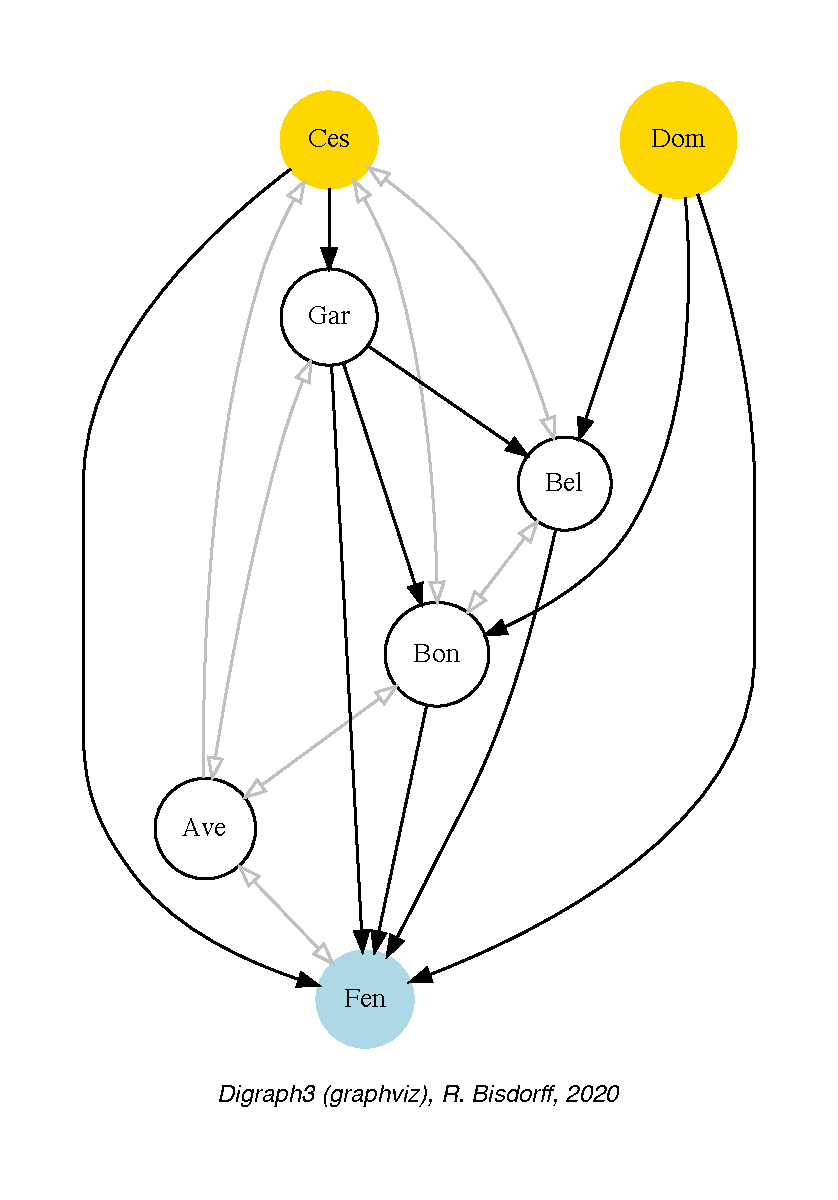
\includegraphics[width=5cm]{Figures/4-3-bestOfficeChoice.pdf}
\caption{Best office choice recommendation from strict outranking digraph. Notice that site \texttt{A} (\emph{Ave}) (the most expensive) is appearing \emph{incomparable} to all the other aternatives}
\label{fig:4.3}       % Give a unique label
\end{figure}
We may finally notice in Listing~\vref{list:4.4} (Lines 16 and 19) that both alternatives \texttt{A} and \texttt{F} are reported as potential worst choice recommendation. Yet, this potential worst choice recommendation appears to be globally indeterminate. This confirms the \emph{incomparability} status of alternative \texttt{A} (see Fig.~\vref{fig:4.3}).
\begin{lstlisting}
>>> gcd = ~(-g) # codual of g
>>> gcd.exportGraphViz(fileName='bestOfficeChoice',\
...                    bestChoice=['C','D'],\
...                    worstChoice=['F'])
  *---- exporting a dot file for GraphViz tools ---------*
   Exporting to bestOfficeChoice.dot
   dot -Grankdir=BT -Tpng bestOfficeChoice.dot \
                    -o bestOfficeChoice.png
\end{lstlisting}

\section{Weakly ordering the outranking digraph}
\label{sec:4.6}

To get a global insight in the overall strict outranking situations, we may use the \texttt{RankingByChoosingDigraph}\index{RankingByChoosingDigraph@\texttt{RankingByChoosingDigraph} class} constructor imported from the \texttt{transitive\-Digraphs}\index{transitiveDigraphs@\texttt{transitiveDigraphs} module} module for computing a \emph{ranking-by-choosing} result from the codual, i.e. the strict outranking digraph instance $gcd$ (see above). If the computing node supports multiple processor cores, \emph{first} and \emph{last} choosing iterations may be run in parallel (see Line 3 in Listing~\vref{list:4.7}).
\begin{figure}[h]
\sidecaption[t]
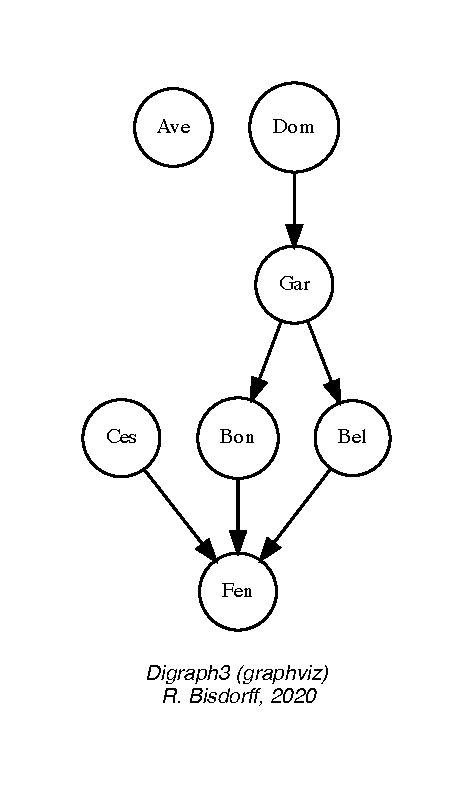
\includegraphics[width=5cm]{Figures/4-4-officeChoiceRanking.pdf}
\caption{In this \emph{ranking-by-choosing} method, where we operate the \emph{epistemic fusion} of iterated (strict) first and last choices, compromise alternative \texttt{D} is now ranked before compromise alternative \texttt{G}. The overall partial ordering result shows again the important fact that the most expensive site \texttt{A}, and the cheapest site \texttt{C}, due to their contradictory performances, appear both \emph{incomparable} with most of the other alternatives.} 
\label{fig:4.4}       % Give a unique label
\end{figure}
\begin{lstlisting}[caption={Ranking-by-choosing the outranking digraph},label=list:4.7]
>>> from transitiveDigraphs import\
...                  RankingByChoosingDigraph
>>> rbc = RankingByChoosingDigraph(gcd)
 Threading ... # multiprocessing if 2 cores are available
 Exiting computing threads
>>> rbc.showRankingByChoosing()
 Ranking by Choosing and Rejecting
    1st ranked ['D']
       2nd ranked ['C', 'G']
       2nd last ranked ['B', 'C', 'E']
    1st last ranked ['A', 'F']
>>> rbc.exportGraphViz('officeChoiceRanking')
 *---- exporting a dot file for GraphViz tools ---------*
  Exporting to officeChoiceRanking.dot
  dot -Grankdir=TB -Tpng officeChoiceRanking.dot\
                   -o officeChoiceRanking.png
\end{lstlisting}
The best choice recommendation appears hence depending on the very importance the CEO is attaching to each of the three decision objectives he is considering. In the given setting here, where he considers that \emph{maximizing the future turnover} is the most important objective followed by \emph{minimizing the Costs} and, less important, \emph{maximizing the working conditions}, site \texttt{D} represents actually the \emph{best compromise}. However, if \emph{Costs} do not play much a role, it would be perhaps better to decide to move to the most advantageous site \texttt{A}; or if, on the contrary, \emph{Costs} do matter a lot, moving to the cheapest alternative \texttt{C} could definitely represent a more convincing recommendation. 

It might be worth editing the criteria significance weights in the\\
\texttt{officeChoice.py} data file in such a way that:
\begin{itemize}
\item All three decision objectives are considered \emph{equally important}, and
\item All criteria under each objective are considered \emph{equi-significant}.
\end{itemize}
What will become the best choice recommendation under this working hypothesis? \footnote{See also the notes of Lecture 7 from the MICS Algorithmic Decision Theory course \citep{ADT-L7}.} 

In the next Chapter~\vref{sec:5} we precisely show how to edit a new performance tableau from a given template file. 

%%%%%%%%%%%%%%%%%%%%%%%%%%%%%%%%%%%%
\phantomsection
\addcontentsline{toc}{section}{Notes}
\section*{Notes}

Following a seminar presentation in 2005 at the LAMSADE\footnote{Laboratoires d'Analyse et de Modélisation de Systèmes d'Aide à la Décision, Université Paris-Dauphine, UMR 7243 CNRS}, where the author promoted the use of kernels of the outranking digraph as suitable candidates for delivering convincing best choice recommendations \citep{BIS-2005}, a critical discussion started about the methodological requirement for a convincing best choice recommendation to be internally stable (pragmatic principle P3). Denis Bouyssou\index{Bouyssou@\textsl{D. Bouyssou}} illustrated his doubts with the example of supposed outranking digraph shown in Fig.~\vref{fig:4.5}.
\begin{figure}[h]
\sidecaption[t]
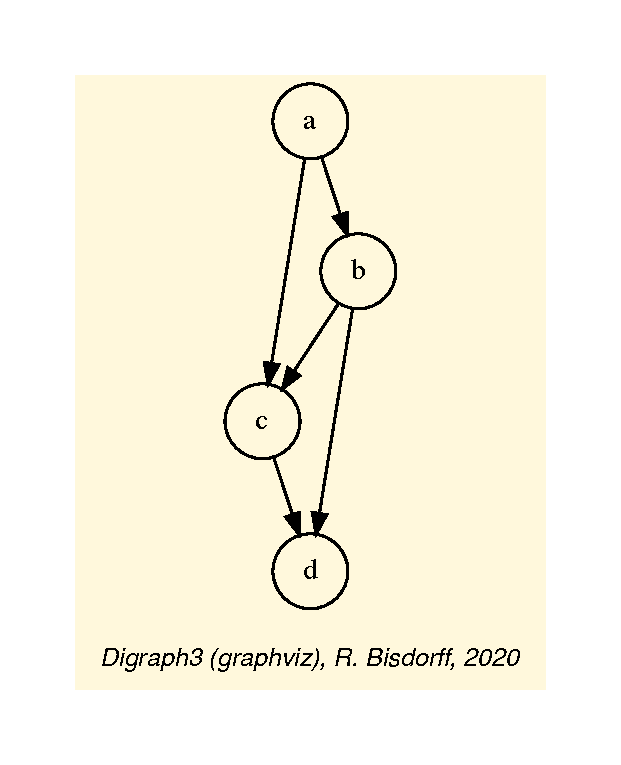
\includegraphics[width=6cm]{Figures/bouyssou11Oct05crisp.pdf}
\caption{The internal stability of a best choice recommendation in question. The only kernel of this digraph is the pair \{a,d\}; yet, it is an ambiguous recommendation, as \{a,d\} is conjointly an outranking and outranked choice. If the instability of the best choice recommendation is, however, not considered a problem then the choice \{a,b\} shows the most convincing strict outranking quality and could be considered in priority for recommendation as potential best choice candidates.}
\label{fig:4.5}       % Give a unique label
\end{figure}

His commentary was the following: Adding alternative \texttt{d} to the set of potential best choice candidates is not convincing as there exists in the given digraph the node \texttt{b}, which is better than \texttt{d}. The argument that the incomparability between \texttt{a} and \texttt{d} should favour \texttt{d} as potential best choice is interesting but another hypothesis could be that \texttt{b} perhaps outranks \texttt{a}. In this latter case, it seams clear that the actual best choice recommendation should be reduced to node \texttt{b}, unless one disposes of other information, like a performance tableau and/or the actual computation method of the outranking situations. In any case, one has to be very clear about the available information when judging a best choice procedure.

It became thereafter clear for us all that both the lack of a specific performance tableau as well as the lack of a precisely defined algorithm for computing valid outranking situations does not allow to judge if a given digraph does indeed model a potential outranking relation. In our present bipolar-valued epistemic approach, a valid outranking digraph instance, following from a given performance tableau and the disjunctive epistemic fusion construction of the outranking relation (see Chapter~\vref{sec:3}), will necessarily verify the weak completeness condition and the coduality principle. As a consequence, incomparability situations are now modelled by epistemic indeterminateness not by the actual absence of a relation.

The digraph proposed by D. Bouyssou in the October 2005 discussion, see Fig.~\vref{fig:4.5}, is effectively not weakly complete and does hence not represent, in our present sense, a valid outranking digraph instance. Yet, it is a partial tournament and as such it may be a strict outranking digraph, i.e. the asymmetric part --the codual-- of a valid outranking digraph. In this case, nodes \texttt{a} and \texttt{d} --the kernel of the strict outranking digraph-- would actually for sure outrank each other and, hence, represent both the natural best choice recommendation. However, in this corresponding \emph{not strict} outranking digraph, node \texttt{a} becomes a \Condorcet winner --outranking for sure all other nodes-- and represents the evident the unique best choice recommendation.

It stays an interesting open mathematical problem to show (or not) that both necessary conditions: --weak completeness and the coduality principle-- are also sufficient for qualifying any bipolar-valued digraph as potential instance of an outranking digraph.


%%%%%%% The chapter bibliography
%\normallatexbib
\clearpage
%\phantomsection
%\addcontentsline{toc}{section}{Chapter Bibliography}
\bibliographystyle{spbasic}
%\typeout{}
\bibliography{03-backMatters/reference}
%\chapter{Computing a best choice recommendation}
\label{sec:6}

\abstract*{To be written.}

\abstract{To be written.}
\begin{quotation}
“... The goal of our research was to design a resolution method ... that is easy to
put into practice, that requires as few and reliable hypotheses as possible, and that
meets the needs [of the decision maker]...” -- \citep*{ROY-1966}.
\end{quotation}

\section{What site to choose ?}
\label{sec:6.1}

A SME, specialized in printing and copy services, has to move into new offices, and its CEO has gathered seven \textbf{potential office sites} (see Table \ref{tab:6.1}).

\begin{table}[h]
\caption{The potential new office sites}
\label{tab:6.1}       % Give a unique label
\begin{center}
  %\begin{small}
    \begin{tabular}{c|l|l|l}
      \svhline\noalign{\smallskip}
      ID & Name & Address & Comment\\
      \noalign{\smallskip}\hline\noalign{\smallskip}
    A &   Ave  &  Avenue de la liberté &  High standing city center\\
    B &   Bon  &  Bonnevoie &             Industrial environment\\
    C &   Ces  &  Cessange &              Residential suburb location\\
    D &   Dom  &  Dommeldange &           Industrial suburb environment\\
    E &   Bel  &  Esch-Belval &           New and ambitious urbanization far from the city\\
    F &   Fen  &  Fentange &              Out in the countryside\\
      G &   Gar  &  Avenue de la Gare &     Main city shopping street\\
      \noalign{\smallskip}\hline
    \end{tabular}
  %\end{small}
\end{center}
\end{table}

Three \textbf{decision objectives} are guiding the CEO's choice:
\begin{enumerate}
\item \emph{minimize} the yearly costs induced by the moving,
\item \emph{maximize} the future turnover of the SME,
\item \emph{maximize} the new working conditions.
\end{enumerate}

The decision consequences to take into account for evaluating the potential new office sites with respect to each of the three objectives are modelled by the following \emph{coherent family of criteria} \footnote{See \citealp{ROY-2000}}.
\begin{table}[h]
\caption{The family of performance criteria}
\label{tab:6.2}       % Give a unique label
\begin{center}
    \begin{tabular}{l|l|l|l}
      \svhline\noalign{\smallskip}
      Objective & ID & Name &  Comment\\
      \noalign{\smallskip}\hline\noalign{\smallskip}
    Yearly costs  &       C &   Costs &       Annual rent, charges, and cleaning\\
    \             &  \      & \        &  \ \\
    Future turnover   &   St &   Standing &    Image and presentation\\
    Future turnover   &   V  &  Visibility &  Circulation of potential customers \\
    Future turnover   &   Pr  & Proximity  &  Distance from town center\\
    \                 &   \   & \          &  \  \\
    Working conditions &  W  &  Space   &     Working space\\
    Working conditions &  Cf &  Comfort  &    Quality of office equipment\\
    Working conditions &  P  &  Parking  &    Available parking facilities\\
      \noalign{\smallskip}\hline
    \end{tabular}   
  \end{center}
\end{table}

The evaluation of the seven potential sites on each criterion are gathered in the following \emph{performance tableau}.
\begin{table}[h]
\caption{Performance evaluations of the potential office sites}
\label{tab:6.3}       % Give a unique label
\begin{center}
    \begin{tabular}{l|c|c|c|c|c|c|c|c}
      \svhline\noalign{\smallskip}
    Criterion  &   weight &  A  &      B &       C &       D &       E &        F &        G\\
       \noalign{\smallskip}\hline\noalign{\smallskip}

    Costs     &    45.0  &   35.0K€ &  17.8K€  & 6.7K€  &  14.1K€ &  34.8K€ &  18.6K€ &  12.0K€\\
    \      &        \    &   \      &  \     &   \     &   \    &    \    &    \    &    \ \\
    Proximity     &     32.0  &   100    &  20 &      80    &   70    &   40    &   0    &    60 \\
    Visibility     &     26.0  &   60     &  80  &     70    &   50    &   60    &   0    &    100 \\
    Standing     &     23.0  &   100   &   10   &    0     &   30    &   90    &   70   &    20 \\
    \        &      \    &   \     &   \    &    \     &   \     &   \     &   \    &    \  \\
    Working space     &     10.0  &   75    &   30   &    0     &   55    &   100   &   0    &    50  \\
    Working comfort     &      6.0  &   0     &   100  &    10    &   30    &   60    &   80   &    50 \\
    Parking     &      3.0  &   90    &   30   &    100   &   90    &   70    &   0    &    80 \\
      \noalign{\smallskip}\hline
    \end{tabular}
  \end{center}
\end{table}

All criteria, except the \emph{Costs} Criterion, admit for grading a qualitative satisfaction scale from $0\%$ (worst) to $100\%$ (best). We may thus notice in Table \ref{tab:6.3} that site 'A' is the most expensive, but also $100\%$ satisfying the \emph{Proximity} as well as the  \emph{Standing} criterion. Whereas the site 'C' is the cheapest one; providing however no satisfaction at all on both the \emph{Standing} and the \emph{Working Space} criteria.

In Table \ref{tab:6.3} we may also notice that the \emph{Costs} criterion admits the highest significance ($45.0$), followed by the \emph{Future turnover} criteria $(32.0 + 26.0 + 23.0 = 81.0)$, The \emph{Working conditions} criteria are the less significant $(10.0 + 6.0, + 3.0 = 19.0)$. It follows that the CEO considers \emph{maximizing the future turnover} the most important objective ($81.0$), followed by minizing the yearly costs ($45.0$), and less important, \emph{maximizing working conditions} ($19.0$). 

Concerning yearly costs, we suppose that the CEO is indifferent up to a performance difference of $1000.00$€, and he actually prefers a site if there is at least a positive difference of $2500.00$€. The grades observed on the six qualitative criteria (measured in percentages of satisfaction) are very subjective and rather imprecise. The CEO is hence indifferent up to a satisfaction difference of $10\%$, and he claims a significant preference when the satisfaction difference is at least of $20\%$.  Furthermore, a satisfaction difference of $80\%$ represents for him a \emph{considerably large} performance difference, triggering the case given a polarisation of the preferential situations (see \citet{BIS-2013}). 

In view of Table \ref{tab:6.3}, what is now the office site we may recommend to the CEO as \textbf{best choice}?

\section{The given performance tableau}
\label{sec:6.2}


A corresponding, \texttt{PerformanceTableau}\index{PerformanceTableau} object, saved in file \texttt{officeChoice.py} is provided in the \texttt{examples} directory of the \Digraph resources. We may inspect its actual content with the computing resources provided by the \texttt{perfTabs}\index{perfTabs} module.
\begin{lstlisting}[caption={Inspecting the \texttt{officeChoice} performance tableau},label=list:6.1]
>>> from perfTabs import PerformanceTableau
>>> t = PerformanceTableau('examples/officeChoice')
>>> t
 *------- PerformanceTableau instance description ------*
   Instance class     : PerformanceTableau
   Instance name      : officeChoice
   Actions            : 7
   Objectives         : 3
   Criteria           : 7
   NaN proportion (%) : 0.0
   Attributes         : ['name', 'actions', 'objectives',
                         'criteria', 'weightPreorder',
			 'NA', 'evaluation']
>>> t.showPerformanceTableau()
 *----  performance tableau -----*
  Criteria|  'C'        'Cf'   'P'   'Pr'   'St'   'V'    'W'   
  Weights |  45.00      6.00   3.00  32.00  23.00  26.00  10.00    
  --------|----------------------------------------------------
   'Ave'  | -35000.00   0.00  90.00 100.00 100.00  60.00  75.00  
   'Bon'  | -17800.00 100.00  30.00  20.00  10.00  80.00  30.00  
   'Ces'  |  -6700.00  10.00 100.00  80.00   0.00  70.00   0.00  
   'Dom'  | -14100.00  30.00  90.00  70.00  30.00  50.00  55.00  
   'Bel'  | -34800.00  60.00  70.00  40.00  90.00  60.00 100.00  
   'Fen'  | -18600.00  80.00   0.00   0.00  70.00   0.00   0.00  
   'Gar'  | -12000.00  50.00  80.00  60.00  20.00 100.00  50.00  
\end{lstlisting}

We thus recover all the input data. To measure the actual preference discrimination we observe on each criterion, we may use the \texttt{showCriteria()}\index{perfTabs!schowCriteria()} method.
\begin{lstlisting}[caption={Inspecting the performance criteria},label=list:6.2]
>>> t.showCriteria(IntegerWeights=True)
 *----  criteria -----*
  C 'Costs'
   Scale = (Decimal('0.00'), Decimal('50000.00'))
   Weight = 45
   Threshold ind : 1000.00 + 0.00x ;  percentile:  9.5
   Threshold pref : 2500.00 + 0.00x ; percentile: 14.3
  Cf 'Comfort'
   Scale = (Decimal('0.00'), Decimal('100.00'))
   Weight = 6
   Threshold ind : 10.00 + 0.00x ;  percentile:   9.5
   Threshold pref : 20.00 + 0.00x ; percentile:  28.6
   Threshold veto : 80.00 + 0.00x ; percentile:  90.5
    ...
\end{lstlisting}

On the \emph{Costs} criterion, $9.5\%$ of the performance differences are considered insignificant and $14.3\%$ below the preference discrimination threshold (see Listing \ref{list:6.2} lines 6-7). On the qualitative \emph{Comfort} criterion, we observe again $9.5\%$ of insignificant performance differences (line 11). Due to the imprecision in the subjective grading, we notice here $28.6\%$ of performance differences below the preference discrimination threshold (Line 12). Furthermore, $100.0 - 90.5 = 9.5\%$ of the performance differences are judged \emph{considerably large} (Line 13); $80\%$ and more of satisfaction differences triggering in fact a polarisation of the preferential situation. Same information is available for all the other criteria. 
 
A colorful comparison of all the performances is shown in Figure \ref{fig:6.1} by the \emph{heatmap}\index{perfTabs!showHTMLPerformanceHeatmap} statistics, illustrating the respective quantile class of each performance. As the set of potential alternatives is tiny, we choose here a classification into performance quintiles.

\begin{lstlisting}
>>> t.showHTMLPerformanceHeatmap(colorLevels=5,\
...                              rankingRule=None)
\end{lstlisting}
    
\begin{figure}[h]
%\sidecaption
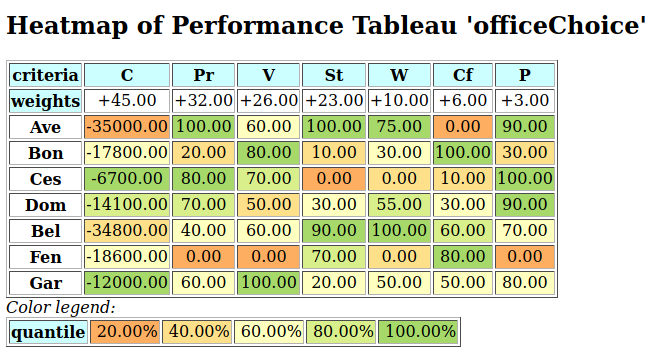
\includegraphics[width=11cm]{Figures/officeChoiceHeatmap.png}
\caption{Unranked heatmap of the office choice performance tableau.}
\label{fig:6.1}       % Give a unique label
\end{figure}

Site $Ave$ shows extreme and contradictory performances: highest \emph{Costs} and no \emph{Working Comfort} on the one hand, and total satisfaction with respect to \emph{Standing}, \emph{Proximity} and \emph{Parking facilities} on the other hand. Similar, but opposite, situation is given for site $Ces$: unsatisfactory \emph{Working Space}, no \emph{Standing} and no \emph{Working Comfort} on the one hand, and lowest \emph{Costs}, best \emph{Proximity} and \emph{Parking facilities} on the other hand. Contrary to these contradictory alternatives, we observe two appealing compromise decision alternatives: sites $Dom$ and $Gar$. Finally, site $Fen$ is clearly the less satisfactory alternative of all.

To help now the CEO choosing the best site, we are going to compute pairwise outrankings on the set of potential sites (see \citet{BIS-2013}).

\section{Computing the outranking digraph}
\label{sec:6.2}

\begin{definition}[Outranking situation]\index{outranking!situation}
For two potential office sites $x$ and $y$:
\begin{itemize}
\item $x$ \emph{outranks} $y$, denoted $(x \succsim y)$, is given when there is:
   \begin{enumerate}
     \item A \emph{majority} of criteria significance concordantly supporting that site $x$ is \emph{at least as satisfactory as} site $y$, and
     \item \emph{No considerable} counter-performance observed on any discordant criterion.      
    \end{enumerate}
\item $x$ \emph{does not outrank} $y$, denoted $(x \not\succsim y)$, is given when there is:
   \begin{enumerate}
    \item A \emph{majority} of criteria concordantly supporting that site $x$ is \emph{not at least as satisfactory as} site $y$, and
    \item \emph{No considerable} better performance observed on any discordant criterion.
    \end{enumerate}
\end{itemize}
\end{definition}
The credibility of each pairwise outranking situation\index{outranking!situation} (see \citet{BIS-2013}), denoted $r(x \succsim y)$, is measured in a bipolar significance valuation $[-1.0, 1.0]$, where \textbf{positive} terms $r(x \succsim y)\, >\, 0.0$ indicate a \textbf{validated}, and \textbf{negative} terms $r(x \succsim y)\, <\, 0.0$ indicate a \textbf{non-validated} outranking situation. The \textbf{median} value $r(x \succsim y)\, = \,0.0$ represents an \textbf{indeterminate} situation (see \citet{BIS-2004a}).   

For computing such a bipolar-valued outranking digraph from the given performance tableau $t$, we use the \texttt{BipolarOutrankingDigraph}\index{outrankingDigraphs!BipolarOutrankingDigraph} constructor from the \texttt{outrankingDigraphs}\index{outrankingDigraphs} module. The corresponding \texttt{showHTMLRelationTable}\index{digraphs!showHTMLRelationTable()} method shows here the resulting bipolar-valued adjacency matrix in a system browser window (see Fig. \ref{fig:6.2}).
\begin{lstlisting}
>>> from outrankingDigraphs import BipolarOutrankingDigraph
>>> g = BipolarOutrankingDigraph(t)
>>> g.showHTMLRelationTable()
\end{lstlisting}
\begin{figure}[h]
%\sidecaption
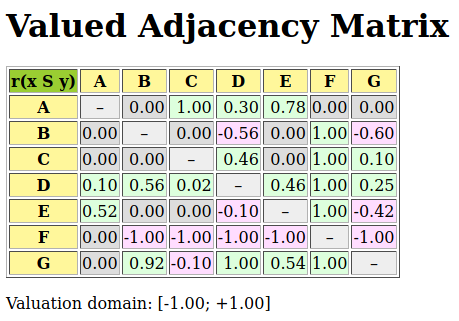
\includegraphics[width=8cm]{Figures/officeChoiceOutranking.png}
\caption{Bipolar-valued adjacency matrix.}
\label{fig:6.2}       % Give a unique label
\end{figure}
In the resulting outranking relation we may notice that Alternative 'D' is \emph{positively outranking} all other potential office sites: 'D' is a \Condorcet winner\index{Condorcet!winner}. Yet, alternatives 'A' (the most expensive) and 'C' (the cheapest) are \emph{not outranked} by any other site; they are in fact \emph{weak} \Condorcet winners.
\begin{lstlisting}
>>> g.computeCondorcetWinners()
 ['D']
>>> g.computeWeakCondorcetWinners()
 ['A', 'C', 'D']
\end{lstlisting}

We may get even more insight in the apparent outranking situations when we draw the corresponding \emph{outranking digraph}\index{outranking!digraph} (see Fig. \ref{fig:6.2}).
\begin{lstlisting}
>>> g.exportGraphViz('officeChoice')
 *---- exporting a dot file for GraphViz tools ---------*
  Exporting to officeChoice.dot
  dot -Grankdir=BT -Tpng officeChoice.dot -o officeChoice.png
\end{lstlisting}
\begin{figure}[h]
\sidecaption
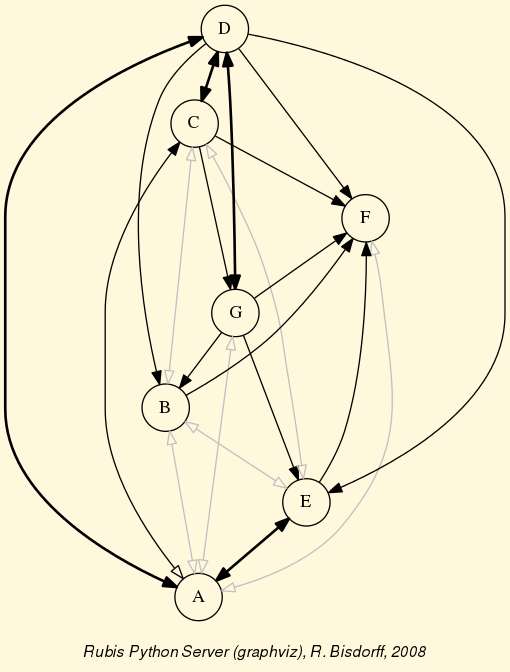
\includegraphics[width=6cm]{Figures/officeChoice.png}
\caption{The office choice outranking digraph.}
\label{fig:6.3}       % Give a unique label
\end{figure}

Outranking digraphs are \emph{weakly complete}\index{weakly complete}, i.e. for all $x$ and $y$ in $X$, $r(x \succsim y)\, <\, 0.0$ implies that $r(y \succsim x)\, \geq\, 0.0$. And, they verify the coduality principle\index{coduality principle}:  $r(x \not\succsim y) \;=\; r(y \succnsim y)$. One may furthermore check that the resulting outranking digraph $g$ here does in fact not admit any cyclic strict preference situation.

\begin{lstlisting}
>>> g.computeChordlessCircuits()
  []
>>> g.showChordlessCircuits()
  No circuits observed in this digraph.
\end{lstlisting}

\section{Computing a \Rubis best choice recommendation}
\label{sec:6.3}

Following the \Rubis outranking method\index{outranking!Rubis best choice recommendation} (see \citet{BIS-2008a}), potential best choice recommendations are determined by the outranking \emph{prekernels}\index{prekernels} --weakly independent and strictly outranking choices-- of the outranking digraph (see the tutorial on computing digraph kernels). The case given, we previously need to break open\index{digraphs!BrokenCocsDigraph} all chordless odd circuits at their weakest link.

\begin{lstlisting}
>>> from digraphs import BrokenCocsDigraph
>>> bcg = BrokenCocsDigraph(g)
>>> bcg.brokenLinks
  set()
\end{lstlisting}

As we observe indeed no such chordless circuits here, we may directly compute the \emph{prekernels} of the outranking digraph $g$.

\begin{lstlisting}[caption={Computing outranking and outranked prekernels},label=list:6.3]
>>> g.showPreKernels()
 *--- Computing preKernels ---*
    Dominant preKernels :
    ['D']
       independence :  1.0
       dominance    :  0.02
       absorbency   :  -1.0
       covering     :  1.000
    ['B', 'E', 'C']
       independence :  0.00
       dominance    :  0.10
       absorbency   :  -1.0
       covering     :  0.500
    ['A', 'G']
       independence :  0.00
       dominance    :  0.78
       absorbency   :  0.00
       covering     :  0.700
    Absorbent preKernels :
    ['F', 'A']
       independence :  0.00
       dominance    :  0.00
       absorbency   :  1.0
       covering     :  0.700
    *----- statistics -----
    graph name:  rel_officeChoice.xml
    number of solutions
     dominant kernels :  3
     absorbent kernels:  1
    cardinality frequency distributions
    cardinality     :  [0, 1, 2, 3, 4, 5, 6, 7]
    dominant kernel :  [0, 1, 1, 1, 0, 0, 0, 0]
    absorbent kernel:  [0, 0, 1, 0, 0, 0, 0, 0]
    Execution time  : 0.00018 sec.
    Results in sets: dompreKernels and abspreKernels.
\end{lstlisting}
  
We notice in Listing \ref{list:6.3} three potential best choice recommendations: the \Condorcet winner 'D' (Line 4), the triplet 'B', 'C' and 'E' (Line 9), and finally the pair 'A' and 'G' (Line 14). The best choice recommendation is now given by the \textbf{most determined} prekernel; the one supported by the most significant criteria coalition. This result is shown with the \texttt{showBestChoiceRecommendation}\index{Digraph!showBestChoiceRecommendation()} method. Notice that this method actually works by default on the broken chords digraph $bcg$.

\begin{lstlisting}[caption={Computing a best choice recommendation},label=list:6.4]
>>> g.showBestChoiceRecommendation(CoDual=False)
 *****************************************
  Rubis best choice recommendation(s) (BCR)
   (in decreasing order of determinateness)   
   Credibility domain: [-1.00,1.00]
    === >> potential best choice(s)
    * choice              : ['D']
      independence        : 1.00
      dominance           : 0.02
      absorbency          : -1.00
      covering (%)        : 100.00
      determinateness (%) : 51.03
      - most credible action(s) = { 'D': 0.02, }
    === >> potential best choice(s)
    * choice              : ['A', 'G']
      independence        : 0.00
      dominance           : 0.78
      absorbency          : 0.00
      covering (%)        : 70.00
      determinateness (%) : 50.00
      - most credible action(s) = { }
    === >> potential best choice(s)
    * choice              : ['B', 'C', 'E']
      independence        : 0.00
      dominance           : 0.10
      absorbency          : -1.00
      covering (%)        : 50.00
      determinateness (%) : 50.00
      - most credible action(s) = { }
    === >> potential worst choice(s) 
    * choice              : ['A', 'F']
      independence        : 0.00
      dominance           : 0.00
      absorbency          : 1.00
      covered (%)         : 70.00
      determinateness (%) : 50.00
      - most credible action(s) = { }
    Execution time: 0.014 seconds
\end{lstlisting}

We notice in Listing \ref{list:6.4} Line 7 above that the most significantly supported best choice recommendation is indeed the \Condorcet winner 'D' supported by a majority of $51.03\%$ of the criteria significance (see Line 12). Both other potential best choice recommendations, as well as the potential worst choice recommendation, are not positively validated as best, resp. worst choices. They may or may not be considered so. Alternative 'A', with extreme contradictory performances, appears both, in a best and a worst choice recommendation (see Lines 15 and 31) and seams hence not actually comparable to its competitors.

\section{Computing \emph{strict best} choice recommendations}
\label{sec:6.4}

When comparing now the performances of alternatives 'D' and 'G' in a pairwise perspective (see below), we notice that, with the given preference discrimination thresholds, alternative 'G' is actually \emph{certainly at least as good as} alternative 'D':  $r(G \succsim D)\, = \, +145/145\, =\, +1.0$.

\begin{lstlisting}[caption={Inspecting pairwise comparisons},label=list:6.5]
>>> g.showPairwiseComparison('G','D')
 *------------  pairwise comparison ----*
  Comparing actions : ('G', 'D')
  crit.  wght.    g(x)      g(y)    diff.  |   ind     pref    concord 	|
   =====================================================================
   'C'  45.00 -12000.00 -14100.00 +2100.00 | 1000.00 2500.00   +45.00 	| 
   'Cf'  6.00     50.00     30.00   +20.00 |   10.00   20.00    +6.00 	| 
   'P'   3.00     80.00     90.00   -10.00 |   10.00   20.00    +3.00 	| 
   'Pr' 32.00     60.00     70.00   -10.00 |   10.00   20.00   +32.00 	| 
   'St' 23.00     20.00     30.00   -10.00 |   10.00   20.00   +23.00 	| 
   'V'  26.00    100.00     50.00   +50.00 |   10.00   20.00   +26.00 	| 
   'W'  10.00     50.00     55.00    -5.00 |   10.00   20.00   +10.00 	|
   =====================================================================
    Valuation in range: -145.00 to +145.00; global concordance: +145.00
\end{lstlisting}

Yet, we must as well notice that the cheapest alternative 'C' is in fact \emph{strictly outranking} alternative 'G':  $r(C \succsim G)\, =\, +15/145\, >\, 0.0$, and $r(G \succsim C)\, =\, -15/145 \,<\, 0.0$.

\begin{lstlisting}
>>> g.showPairwiseComparison('C','G')
 *------------  pairwise comparison ----*
  Comparing actions : ('C','G')/('G','C')
  crit. wght.   g(x)     g(y)      diff.  |   ind.   pref. ('C','G')/('G','C')|
   ===========================================================================
   'C'   45.00 -6700.00 -12000.00 +5300.00 | 1000.00 2500.00    +45.00/-45.00 | 
   'Cf'   6.00    10.00     50.00   -40.00 |   10.00   20.00     -6.00/ +6.00 | 
   'P'    3.00   100.00     80.00   +20.00 |   10.00   20.00     +3.00/ -3.00 | 
   'Pr'  32.00    80.00     60.00   +20.00 |   10.00   20.00    +32.00/-32.00 | 
   'St'  23.00     0.00     20.00   -20.00 |   10.00   20.00    -23.00/+23.00 | 
   'V'   26.00    70.00    100.00   -30.00 |   10.00   20.00    -26.00/+26.00 | 
   'W'   10.00     0.00     50.00   -50.00 |   10.00   20.00    -10.00/+10.00 |
   ===========================================================================
    Valuation in range: -145.00 to +145.00; global concordance: +15.00/-15.00
\end{lstlisting}
  
To model these \emph{strict outranking} situations\index{strict outranking!situation}, we may recompute the best choice recommendation on the \textbf{codual}, the converse ($\sim$) of the dual ($-$)\footnote{Not to be confused with the dual graph of a plane graph $g$ that has a vertex for each face of $g$. Here we mean the \emph{less than} (strict converse) relation corresponding to a \emph{greater or equal} relation, or the \emph{less than or equal} relation corresponding to a (strict) \emph{better than} relation.}, of the outranking digraph instance $g$ (see \citet{BIS-2013}]), as follows:
\begin{lstlisting}[caption={Computing the strict best choice recommendation},label=list:6.6]
>>> g.showBestChoiceRecommendation(\
...                   CoDual=True,\
...                   ChoiceVector=True)   
* --- Best and worst choice recommendation(s) ---*
  (in decreasing order of determinateness)   
  Credibility domain: [-1.00,1.00]
    === >> potential best choice(s)
    * choice              : ['A', 'C', 'D']
      independence        : 0.00
      dominance           : 0.10
      absorbency          : 0.00
      covering (%)        : 41.67
      determinateness (%) : 50.59
      - characteristic vector = {
             'D': 0.02, 'G': 0.00, 'C': 0.00,
	     'A': 0.00, 'F': -0.02, 'E': -0.02, 'B': -0.02, }
    === >> potential worst choice(s) 
    * choice              : ['A', 'F']
      independence        : 0.00
      dominance           : -0.52
      absorbency          : 1.00
      covered (%)         : 50.00
      determinateness (%) : 50.00
      - characteristic vector = { 'G': 0.00, 'F': 0.00, 'E': 0.00,
	     'D': 0.00, 'C': 0.00, 'B': 0.00, 'A': 0.00, }
\end{lstlisting}				  

It is interesting to notice in Listing \ref{list:6.6} Line 9 that the \emph{strict best choice recommendation} consists in the set of weak \Condorcet winners\index{Condorcet!winner}: 'A', 'C' and 'D'. In the corresponding characteristic vector (see Lines 15-16), representing the bipolar credibility degree with which each alternative may indeed be considered a best choice (see \citet{BIS-2006a,BIS-2006b}), we find confirmed that alternative 'D' is the only positively validated one, whereas both extreme alternatives - 'A' (the most expensive) and 'C' (the cheapest) - stay in an indeterminate situation. They may be potential best choice candidates besides 'D'. Notice furthermore that compromise alternative $G$, while not actually included in any outranking prekernel, shows as well an indeterminate situation with respect to \emph{being or not being} a potential best choice candidate. 

We may also notice (see Line 16 and Line 19) that both alternatives 'A' and 'F' are reported as certainly strict outranked choices, hence as \emph{potential worst choice recommendation} . This confirms again the global incomparability status of alternative 'A' (see Fig. \ref{fig:6.3}).

\begin{lstlisting}
>>> gcd = ~(-g) # codual of g
>>> gcd.exportGraphViz(fileName='bestChoiceChoice',\
...                    bestChoice=['A','C','D'],\
...                    worstChoice=['F'])
 *---- exporting a dot file for GraphViz tools ---------*
  Exporting to bestOfficeChoice.dot
  dot -Grankdir=BT -Tpng bestOfficeChoice.dot -o bestOfficeChoice.png
\end{lstlisting}

\begin{figure}[h]
\sidecaption
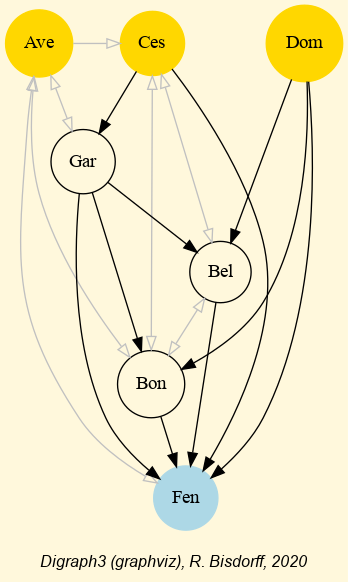
\includegraphics[width=5cm]{Figures/bestOfficeChoice.png}
\caption{Best office choice recommendation from strict outranking digraph.}
\label{fig:6.4}       % Give a unique label
\end{figure}

\section{Weakly ordering the outranking digraph}
\label{sec:6.6}

To get a more complete insight in the overall strict outranking situations, we may use the \texttt{RankingByChoosingDigraph} constructor imported from the \texttt{transitiveDigraphs} module for computing a \textbf{ranking-by-choosing} result from the codual, i.e. the strict outranking digraph instance $gcd$ (see above). If the computing node supports multiple processor cores, best and worst choosing iterations are run in parallel (see Line 3 below).

\begin{lstlisting}
>>> from transitiveDigraphs import RankingByChoosingDigraph
>>> rbc = RankingByChoosingDigraph(gcd)
 Threading ...  # multiprocessing if 2 cores are available
 Exiting computing threads
>>> rbc.showRankingByChoosing()
 Ranking by Choosing and Rejecting
    1st ranked ['D']
       2nd ranked ['C', 'G']
       2nd last ranked ['B', 'C', 'E']
    1st last ranked ['A', 'F']
>>> rbc.exportGraphViz('officeChoiceRanking')
 *---- exporting a dot file for GraphViz tools ---------*
  Exporting to officeChoiceRanking.dot
  dot -Grankdir=TB -Tpng officeChoiceRanking.dot\
                   -o officeChoiceRanking.png
\end{lstlisting}

\begin{figure}[h]
\sidecaption
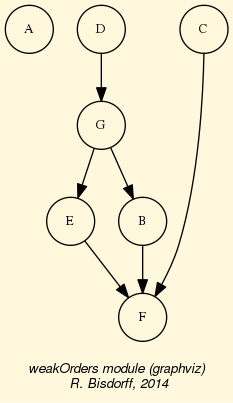
\includegraphics[width=6cm]{Figures/officeChoiceRanking.png}
\caption{In this \textbf{ranking-by-choosing} method, where we operate the \emph{epistemic fusion} of iterated (strict) best and worst choices, compromise alternative $D$ is now ranked before compromise alternative $G$. The overall partial ordering result shows again the important fact that the most expensive site $A$, and the cheapest site $C$, both appear incomparable with most of the other alternatives, as is apparent from the Hasse diagram of the ranking-by-choosing result here.} 
\label{fig:6.5}       % Give a unique label
\end{figure}
	   
The best choice recommendation appears hence depending on the very importance the CEO is attaching to each of the three decision objectives he is considering. In the setting here, where he considers that \emph{maximizing the future turnover} is the most important objective followed by \emph{minimizing the Costs} and, less important, \emph{maximizing the working conditions}, site $D$ represents actually the best compromise. However, if \emph{Costs} do not play much a role, it would be perhaps better to decide to move to the most advantageous site $A$; or if, on the contrary, \emph{Costs} do matter a lot, moving to the cheapest alternative $C$ could definitely represent a more convincing recommendation. 

\noindent \textbf{Exercise:}

\noindent It might be worth modifying these criteria significance weights in the \texttt{officeChoice.py} data file in such a way that:
\begin{itemize}
\item All criteria under an objective appear \emph{equi-significant}, and
\item All three decision objectives are considered \emph{equally important}.
\end{itemize}
What will become the best choice recommendation under this working hypothesis? \footnote{See also Lecture 7 notes from the MICS Algorithmic Decision Theory course \citep{ADT-L7}.} 


%%%%%%% The chapter bibliography
%\normallatexbib
\clearpage
%\phantomsection
%\addcontentsline{toc}{section}{Chapter Bibliography}
\bibliographystyle{spbasic}
%\typeout{}
\bibliography{03-backMatters/reference}
%\chapter{Computing a best choice recommendation}
\label{sec:6}

\abstract*{To be written.}

\abstract{To be written.}
\begin{quotation}
“... The goal of our research was to design a resolution method ... that is easy to
put into practice, that requires as few and reliable hypotheses as possible, and that
meets the needs [of the decision maker]...” -- \citep*{ROY-1966}.
\end{quotation}

\section{What site to choose ?}
\label{sec:6.1}

A SME, specialized in printing and copy services, has to move into new offices, and its CEO has gathered seven \textbf{potential office sites} (see Table \ref{tab:6.1}).

\begin{table}[h]
\caption{The potential new office sites}
\label{tab:6.1}       % Give a unique label
\begin{center}
  %\begin{small}
    \begin{tabular}{c|l|l|l}
      \svhline\noalign{\smallskip}
      ID & Name & Address & Comment\\
      \noalign{\smallskip}\hline\noalign{\smallskip}
    A &   Ave  &  Avenue de la liberté &  High standing city center\\
    B &   Bon  &  Bonnevoie &             Industrial environment\\
    C &   Ces  &  Cessange &              Residential suburb location\\
    D &   Dom  &  Dommeldange &           Industrial suburb environment\\
    E &   Bel  &  Esch-Belval &           New and ambitious urbanization far from the city\\
    F &   Fen  &  Fentange &              Out in the countryside\\
      G &   Gar  &  Avenue de la Gare &     Main city shopping street\\
      \noalign{\smallskip}\hline
    \end{tabular}
  %\end{small}
\end{center}
\end{table}

Three \textbf{decision objectives} are guiding the CEO's choice:
\begin{enumerate}
\item \emph{minimize} the yearly costs induced by the moving,
\item \emph{maximize} the future turnover of the SME,
\item \emph{maximize} the new working conditions.
\end{enumerate}

The decision consequences to take into account for evaluating the potential new office sites with respect to each of the three objectives are modelled by the following \emph{coherent family of criteria} \footnote{See \citealp{ROY-2000}}.
\begin{table}[h]
\caption{The family of performance criteria}
\label{tab:6.2}       % Give a unique label
\begin{center}
    \begin{tabular}{l|l|l|l}
      \svhline\noalign{\smallskip}
      Objective & ID & Name &  Comment\\
      \noalign{\smallskip}\hline\noalign{\smallskip}
    Yearly costs  &       C &   Costs &       Annual rent, charges, and cleaning\\
    \             &  \      & \        &  \ \\
    Future turnover   &   St &   Standing &    Image and presentation\\
    Future turnover   &   V  &  Visibility &  Circulation of potential customers \\
    Future turnover   &   Pr  & Proximity  &  Distance from town center\\
    \                 &   \   & \          &  \  \\
    Working conditions &  W  &  Space   &     Working space\\
    Working conditions &  Cf &  Comfort  &    Quality of office equipment\\
    Working conditions &  P  &  Parking  &    Available parking facilities\\
      \noalign{\smallskip}\hline
    \end{tabular}   
  \end{center}
\end{table}

The evaluation of the seven potential sites on each criterion are gathered in the following \emph{performance tableau}.
\begin{table}[h]
\caption{Performance evaluations of the potential office sites}
\label{tab:6.3}       % Give a unique label
\begin{center}
    \begin{tabular}{l|c|c|c|c|c|c|c|c}
      \svhline\noalign{\smallskip}
    Criterion  &   weight &  A  &      B &       C &       D &       E &        F &        G\\
       \noalign{\smallskip}\hline\noalign{\smallskip}

    Costs     &    45.0  &   35.0K€ &  17.8K€  & 6.7K€  &  14.1K€ &  34.8K€ &  18.6K€ &  12.0K€\\
    \      &        \    &   \      &  \     &   \     &   \    &    \    &    \    &    \ \\
    Proximity     &     32.0  &   100    &  20 &      80    &   70    &   40    &   0    &    60 \\
    Visibility     &     26.0  &   60     &  80  &     70    &   50    &   60    &   0    &    100 \\
    Standing     &     23.0  &   100   &   10   &    0     &   30    &   90    &   70   &    20 \\
    \        &      \    &   \     &   \    &    \     &   \     &   \     &   \    &    \  \\
    Working space     &     10.0  &   75    &   30   &    0     &   55    &   100   &   0    &    50  \\
    Working comfort     &      6.0  &   0     &   100  &    10    &   30    &   60    &   80   &    50 \\
    Parking     &      3.0  &   90    &   30   &    100   &   90    &   70    &   0    &    80 \\
      \noalign{\smallskip}\hline
    \end{tabular}
  \end{center}
\end{table}

All criteria, except the \emph{Costs} Criterion, admit for grading a qualitative satisfaction scale from $0\%$ (worst) to $100\%$ (best). We may thus notice in Table \ref{tab:6.3} that site 'A' is the most expensive, but also $100\%$ satisfying the \emph{Proximity} as well as the  \emph{Standing} criterion. Whereas the site 'C' is the cheapest one; providing however no satisfaction at all on both the \emph{Standing} and the \emph{Working Space} criteria.

In Table \ref{tab:6.3} we may also notice that the \emph{Costs} criterion admits the highest significance ($45.0$), followed by the \emph{Future turnover} criteria $(32.0 + 26.0 + 23.0 = 81.0)$, The \emph{Working conditions} criteria are the less significant $(10.0 + 6.0, + 3.0 = 19.0)$. It follows that the CEO considers \emph{maximizing the future turnover} the most important objective ($81.0$), followed by minizing the yearly costs ($45.0$), and less important, \emph{maximizing working conditions} ($19.0$). 

Concerning yearly costs, we suppose that the CEO is indifferent up to a performance difference of $1000.00$€, and he actually prefers a site if there is at least a positive difference of $2500.00$€. The grades observed on the six qualitative criteria (measured in percentages of satisfaction) are very subjective and rather imprecise. The CEO is hence indifferent up to a satisfaction difference of $10\%$, and he claims a significant preference when the satisfaction difference is at least of $20\%$.  Furthermore, a satisfaction difference of $80\%$ represents for him a \emph{considerably large} performance difference, triggering the case given a polarisation of the preferential situations (see \citet{BIS-2013}). 

In view of Table \ref{tab:6.3}, what is now the office site we may recommend to the CEO as \textbf{best choice}?

\section{The given performance tableau}
\label{sec:6.2}


A corresponding, \texttt{PerformanceTableau}\index{PerformanceTableau} object, saved in file \texttt{officeChoice.py} is provided in the \texttt{examples} directory of the \Digraph resources. We may inspect its actual content with the computing resources provided by the \texttt{perfTabs}\index{perfTabs} module.
\begin{lstlisting}[caption={Inspecting the \texttt{officeChoice} performance tableau},label=list:6.1]
>>> from perfTabs import PerformanceTableau
>>> t = PerformanceTableau('examples/officeChoice')
>>> t
 *------- PerformanceTableau instance description ------*
   Instance class     : PerformanceTableau
   Instance name      : officeChoice
   Actions            : 7
   Objectives         : 3
   Criteria           : 7
   NaN proportion (%) : 0.0
   Attributes         : ['name', 'actions', 'objectives',
                         'criteria', 'weightPreorder',
			 'NA', 'evaluation']
>>> t.showPerformanceTableau()
 *----  performance tableau -----*
  Criteria|  'C'        'Cf'   'P'   'Pr'   'St'   'V'    'W'   
  Weights |  45.00      6.00   3.00  32.00  23.00  26.00  10.00    
  --------|----------------------------------------------------
   'Ave'  | -35000.00   0.00  90.00 100.00 100.00  60.00  75.00  
   'Bon'  | -17800.00 100.00  30.00  20.00  10.00  80.00  30.00  
   'Ces'  |  -6700.00  10.00 100.00  80.00   0.00  70.00   0.00  
   'Dom'  | -14100.00  30.00  90.00  70.00  30.00  50.00  55.00  
   'Bel'  | -34800.00  60.00  70.00  40.00  90.00  60.00 100.00  
   'Fen'  | -18600.00  80.00   0.00   0.00  70.00   0.00   0.00  
   'Gar'  | -12000.00  50.00  80.00  60.00  20.00 100.00  50.00  
\end{lstlisting}

We thus recover all the input data. To measure the actual preference discrimination we observe on each criterion, we may use the \texttt{showCriteria()}\index{perfTabs!schowCriteria()} method.
\begin{lstlisting}[caption={Inspecting the performance criteria},label=list:6.2]
>>> t.showCriteria(IntegerWeights=True)
 *----  criteria -----*
  C 'Costs'
   Scale = (Decimal('0.00'), Decimal('50000.00'))
   Weight = 45
   Threshold ind : 1000.00 + 0.00x ;  percentile:  9.5
   Threshold pref : 2500.00 + 0.00x ; percentile: 14.3
  Cf 'Comfort'
   Scale = (Decimal('0.00'), Decimal('100.00'))
   Weight = 6
   Threshold ind : 10.00 + 0.00x ;  percentile:   9.5
   Threshold pref : 20.00 + 0.00x ; percentile:  28.6
   Threshold veto : 80.00 + 0.00x ; percentile:  90.5
    ...
\end{lstlisting}

On the \emph{Costs} criterion, $9.5\%$ of the performance differences are considered insignificant and $14.3\%$ below the preference discrimination threshold (see Listing \ref{list:6.2} lines 6-7). On the qualitative \emph{Comfort} criterion, we observe again $9.5\%$ of insignificant performance differences (line 11). Due to the imprecision in the subjective grading, we notice here $28.6\%$ of performance differences below the preference discrimination threshold (Line 12). Furthermore, $100.0 - 90.5 = 9.5\%$ of the performance differences are judged \emph{considerably large} (Line 13); $80\%$ and more of satisfaction differences triggering in fact a polarisation of the preferential situation. Same information is available for all the other criteria. 
 
A colorful comparison of all the performances is shown in Figure \ref{fig:6.1} by the \emph{heatmap}\index{perfTabs!showHTMLPerformanceHeatmap} statistics, illustrating the respective quantile class of each performance. As the set of potential alternatives is tiny, we choose here a classification into performance quintiles.

\begin{lstlisting}
>>> t.showHTMLPerformanceHeatmap(colorLevels=5,\
...                              rankingRule=None)
\end{lstlisting}
    
\begin{figure}[h]
%\sidecaption
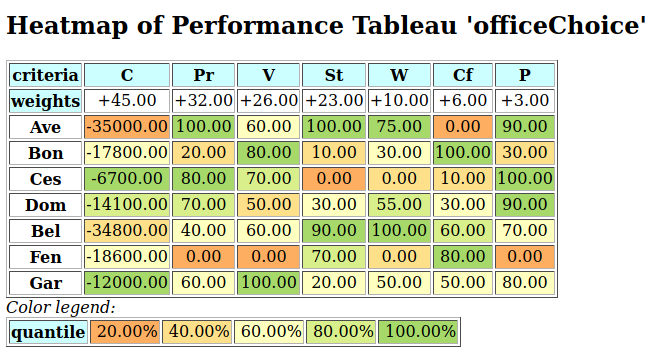
\includegraphics[width=11cm]{Figures/officeChoiceHeatmap.png}
\caption{Unranked heatmap of the office choice performance tableau.}
\label{fig:6.1}       % Give a unique label
\end{figure}

Site $Ave$ shows extreme and contradictory performances: highest \emph{Costs} and no \emph{Working Comfort} on the one hand, and total satisfaction with respect to \emph{Standing}, \emph{Proximity} and \emph{Parking facilities} on the other hand. Similar, but opposite, situation is given for site $Ces$: unsatisfactory \emph{Working Space}, no \emph{Standing} and no \emph{Working Comfort} on the one hand, and lowest \emph{Costs}, best \emph{Proximity} and \emph{Parking facilities} on the other hand. Contrary to these contradictory alternatives, we observe two appealing compromise decision alternatives: sites $Dom$ and $Gar$. Finally, site $Fen$ is clearly the less satisfactory alternative of all.

To help now the CEO choosing the best site, we are going to compute pairwise outrankings on the set of potential sites (see \citet{BIS-2013}).

\section{Computing the outranking digraph}
\label{sec:6.2}

\begin{definition}[Outranking situation]\index{outranking!situation}
For two potential office sites $x$ and $y$:
\begin{itemize}
\item $x$ \emph{outranks} $y$, denoted $(x \succsim y)$, is given when there is:
   \begin{enumerate}
     \item A \emph{majority} of criteria significance concordantly supporting that site $x$ is \emph{at least as satisfactory as} site $y$, and
     \item \emph{No considerable} counter-performance observed on any discordant criterion.      
    \end{enumerate}
\item $x$ \emph{does not outrank} $y$, denoted $(x \not\succsim y)$, is given when there is:
   \begin{enumerate}
    \item A \emph{majority} of criteria concordantly supporting that site $x$ is \emph{not at least as satisfactory as} site $y$, and
    \item \emph{No considerable} better performance observed on any discordant criterion.
    \end{enumerate}
\end{itemize}
\end{definition}
The credibility of each pairwise outranking situation\index{outranking!situation} (see \citet{BIS-2013}), denoted $r(x \succsim y)$, is measured in a bipolar significance valuation $[-1.0, 1.0]$, where \textbf{positive} terms $r(x \succsim y)\, >\, 0.0$ indicate a \textbf{validated}, and \textbf{negative} terms $r(x \succsim y)\, <\, 0.0$ indicate a \textbf{non-validated} outranking situation. The \textbf{median} value $r(x \succsim y)\, = \,0.0$ represents an \textbf{indeterminate} situation (see \citet{BIS-2004a}).   

For computing such a bipolar-valued outranking digraph from the given performance tableau $t$, we use the \texttt{BipolarOutrankingDigraph}\index{outrankingDigraphs!BipolarOutrankingDigraph} constructor from the \texttt{outrankingDigraphs}\index{outrankingDigraphs} module. The corresponding \texttt{showHTMLRelationTable}\index{digraphs!showHTMLRelationTable()} method shows here the resulting bipolar-valued adjacency matrix in a system browser window (see Fig. \ref{fig:6.2}).
\begin{lstlisting}
>>> from outrankingDigraphs import BipolarOutrankingDigraph
>>> g = BipolarOutrankingDigraph(t)
>>> g.showHTMLRelationTable()
\end{lstlisting}
\begin{figure}[h]
%\sidecaption
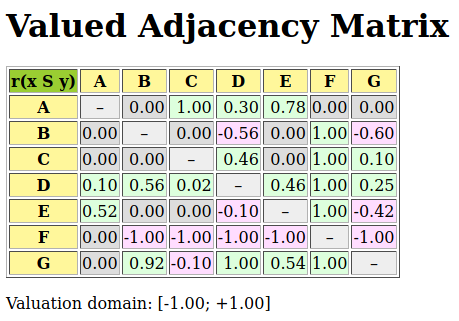
\includegraphics[width=8cm]{Figures/officeChoiceOutranking.png}
\caption{Bipolar-valued adjacency matrix.}
\label{fig:6.2}       % Give a unique label
\end{figure}
In the resulting outranking relation we may notice that Alternative 'D' is \emph{positively outranking} all other potential office sites: 'D' is a \Condorcet winner\index{Condorcet!winner}. Yet, alternatives 'A' (the most expensive) and 'C' (the cheapest) are \emph{not outranked} by any other site; they are in fact \emph{weak} \Condorcet winners.
\begin{lstlisting}
>>> g.computeCondorcetWinners()
 ['D']
>>> g.computeWeakCondorcetWinners()
 ['A', 'C', 'D']
\end{lstlisting}

We may get even more insight in the apparent outranking situations when we draw the corresponding \emph{outranking digraph}\index{outranking!digraph} (see Fig. \ref{fig:6.2}).
\begin{lstlisting}
>>> g.exportGraphViz('officeChoice')
 *---- exporting a dot file for GraphViz tools ---------*
  Exporting to officeChoice.dot
  dot -Grankdir=BT -Tpng officeChoice.dot -o officeChoice.png
\end{lstlisting}
\begin{figure}[h]
\sidecaption
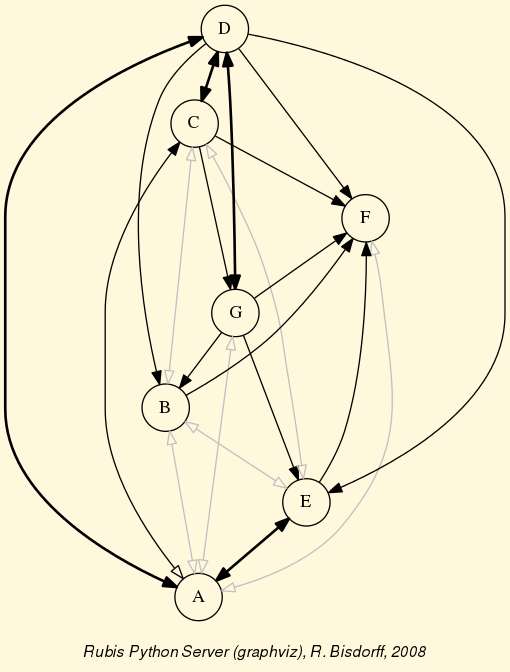
\includegraphics[width=6cm]{Figures/officeChoice.png}
\caption{The office choice outranking digraph.}
\label{fig:6.3}       % Give a unique label
\end{figure}

Outranking digraphs are \emph{weakly complete}\index{weakly complete}, i.e. for all $x$ and $y$ in $X$, $r(x \succsim y)\, <\, 0.0$ implies that $r(y \succsim x)\, \geq\, 0.0$. And, they verify the coduality principle\index{coduality principle}:  $r(x \not\succsim y) \;=\; r(y \succnsim y)$. One may furthermore check that the resulting outranking digraph $g$ here does in fact not admit any cyclic strict preference situation.

\begin{lstlisting}
>>> g.computeChordlessCircuits()
  []
>>> g.showChordlessCircuits()
  No circuits observed in this digraph.
\end{lstlisting}

\section{Computing a \Rubis best choice recommendation}
\label{sec:6.3}

Following the \Rubis outranking method\index{outranking!Rubis best choice recommendation} (see \citet{BIS-2008a}), potential best choice recommendations are determined by the outranking \emph{prekernels}\index{prekernels} --weakly independent and strictly outranking choices-- of the outranking digraph (see the tutorial on computing digraph kernels). The case given, we previously need to break open\index{digraphs!BrokenCocsDigraph} all chordless odd circuits at their weakest link.

\begin{lstlisting}
>>> from digraphs import BrokenCocsDigraph
>>> bcg = BrokenCocsDigraph(g)
>>> bcg.brokenLinks
  set()
\end{lstlisting}

As we observe indeed no such chordless circuits here, we may directly compute the \emph{prekernels} of the outranking digraph $g$.

\begin{lstlisting}[caption={Computing outranking and outranked prekernels},label=list:6.3]
>>> g.showPreKernels()
 *--- Computing preKernels ---*
    Dominant preKernels :
    ['D']
       independence :  1.0
       dominance    :  0.02
       absorbency   :  -1.0
       covering     :  1.000
    ['B', 'E', 'C']
       independence :  0.00
       dominance    :  0.10
       absorbency   :  -1.0
       covering     :  0.500
    ['A', 'G']
       independence :  0.00
       dominance    :  0.78
       absorbency   :  0.00
       covering     :  0.700
    Absorbent preKernels :
    ['F', 'A']
       independence :  0.00
       dominance    :  0.00
       absorbency   :  1.0
       covering     :  0.700
    *----- statistics -----
    graph name:  rel_officeChoice.xml
    number of solutions
     dominant kernels :  3
     absorbent kernels:  1
    cardinality frequency distributions
    cardinality     :  [0, 1, 2, 3, 4, 5, 6, 7]
    dominant kernel :  [0, 1, 1, 1, 0, 0, 0, 0]
    absorbent kernel:  [0, 0, 1, 0, 0, 0, 0, 0]
    Execution time  : 0.00018 sec.
    Results in sets: dompreKernels and abspreKernels.
\end{lstlisting}
  
We notice in Listing \ref{list:6.3} three potential best choice recommendations: the \Condorcet winner 'D' (Line 4), the triplet 'B', 'C' and 'E' (Line 9), and finally the pair 'A' and 'G' (Line 14). The best choice recommendation is now given by the \textbf{most determined} prekernel; the one supported by the most significant criteria coalition. This result is shown with the \texttt{showBestChoiceRecommendation}\index{Digraph!showBestChoiceRecommendation()} method. Notice that this method actually works by default on the broken chords digraph $bcg$.

\begin{lstlisting}[caption={Computing a best choice recommendation},label=list:6.4]
>>> g.showBestChoiceRecommendation(CoDual=False)
 *****************************************
  Rubis best choice recommendation(s) (BCR)
   (in decreasing order of determinateness)   
   Credibility domain: [-1.00,1.00]
    === >> potential best choice(s)
    * choice              : ['D']
      independence        : 1.00
      dominance           : 0.02
      absorbency          : -1.00
      covering (%)        : 100.00
      determinateness (%) : 51.03
      - most credible action(s) = { 'D': 0.02, }
    === >> potential best choice(s)
    * choice              : ['A', 'G']
      independence        : 0.00
      dominance           : 0.78
      absorbency          : 0.00
      covering (%)        : 70.00
      determinateness (%) : 50.00
      - most credible action(s) = { }
    === >> potential best choice(s)
    * choice              : ['B', 'C', 'E']
      independence        : 0.00
      dominance           : 0.10
      absorbency          : -1.00
      covering (%)        : 50.00
      determinateness (%) : 50.00
      - most credible action(s) = { }
    === >> potential worst choice(s) 
    * choice              : ['A', 'F']
      independence        : 0.00
      dominance           : 0.00
      absorbency          : 1.00
      covered (%)         : 70.00
      determinateness (%) : 50.00
      - most credible action(s) = { }
    Execution time: 0.014 seconds
\end{lstlisting}

We notice in Listing \ref{list:6.4} Line 7 above that the most significantly supported best choice recommendation is indeed the \Condorcet winner 'D' supported by a majority of $51.03\%$ of the criteria significance (see Line 12). Both other potential best choice recommendations, as well as the potential worst choice recommendation, are not positively validated as best, resp. worst choices. They may or may not be considered so. Alternative 'A', with extreme contradictory performances, appears both, in a best and a worst choice recommendation (see Lines 15 and 31) and seams hence not actually comparable to its competitors.

\section{Computing \emph{strict best} choice recommendations}
\label{sec:6.4}

When comparing now the performances of alternatives 'D' and 'G' in a pairwise perspective (see below), we notice that, with the given preference discrimination thresholds, alternative 'G' is actually \emph{certainly at least as good as} alternative 'D':  $r(G \succsim D)\, = \, +145/145\, =\, +1.0$.

\begin{lstlisting}[caption={Inspecting pairwise comparisons},label=list:6.5]
>>> g.showPairwiseComparison('G','D')
 *------------  pairwise comparison ----*
  Comparing actions : ('G', 'D')
  crit.  wght.    g(x)      g(y)    diff.  |   ind     pref    concord 	|
   =====================================================================
   'C'  45.00 -12000.00 -14100.00 +2100.00 | 1000.00 2500.00   +45.00 	| 
   'Cf'  6.00     50.00     30.00   +20.00 |   10.00   20.00    +6.00 	| 
   'P'   3.00     80.00     90.00   -10.00 |   10.00   20.00    +3.00 	| 
   'Pr' 32.00     60.00     70.00   -10.00 |   10.00   20.00   +32.00 	| 
   'St' 23.00     20.00     30.00   -10.00 |   10.00   20.00   +23.00 	| 
   'V'  26.00    100.00     50.00   +50.00 |   10.00   20.00   +26.00 	| 
   'W'  10.00     50.00     55.00    -5.00 |   10.00   20.00   +10.00 	|
   =====================================================================
    Valuation in range: -145.00 to +145.00; global concordance: +145.00
\end{lstlisting}

Yet, we must as well notice that the cheapest alternative 'C' is in fact \emph{strictly outranking} alternative 'G':  $r(C \succsim G)\, =\, +15/145\, >\, 0.0$, and $r(G \succsim C)\, =\, -15/145 \,<\, 0.0$.

\begin{lstlisting}
>>> g.showPairwiseComparison('C','G')
 *------------  pairwise comparison ----*
  Comparing actions : ('C','G')/('G','C')
  crit. wght.   g(x)     g(y)      diff.  |   ind.   pref. ('C','G')/('G','C')|
   ===========================================================================
   'C'   45.00 -6700.00 -12000.00 +5300.00 | 1000.00 2500.00    +45.00/-45.00 | 
   'Cf'   6.00    10.00     50.00   -40.00 |   10.00   20.00     -6.00/ +6.00 | 
   'P'    3.00   100.00     80.00   +20.00 |   10.00   20.00     +3.00/ -3.00 | 
   'Pr'  32.00    80.00     60.00   +20.00 |   10.00   20.00    +32.00/-32.00 | 
   'St'  23.00     0.00     20.00   -20.00 |   10.00   20.00    -23.00/+23.00 | 
   'V'   26.00    70.00    100.00   -30.00 |   10.00   20.00    -26.00/+26.00 | 
   'W'   10.00     0.00     50.00   -50.00 |   10.00   20.00    -10.00/+10.00 |
   ===========================================================================
    Valuation in range: -145.00 to +145.00; global concordance: +15.00/-15.00
\end{lstlisting}
  
To model these \emph{strict outranking} situations\index{strict outranking!situation}, we may recompute the best choice recommendation on the \textbf{codual}, the converse ($\sim$) of the dual ($-$)\footnote{Not to be confused with the dual graph of a plane graph $g$ that has a vertex for each face of $g$. Here we mean the \emph{less than} (strict converse) relation corresponding to a \emph{greater or equal} relation, or the \emph{less than or equal} relation corresponding to a (strict) \emph{better than} relation.}, of the outranking digraph instance $g$ (see \citet{BIS-2013}]), as follows:
\begin{lstlisting}[caption={Computing the strict best choice recommendation},label=list:6.6]
>>> g.showBestChoiceRecommendation(\
...                   CoDual=True,\
...                   ChoiceVector=True)   
* --- Best and worst choice recommendation(s) ---*
  (in decreasing order of determinateness)   
  Credibility domain: [-1.00,1.00]
    === >> potential best choice(s)
    * choice              : ['A', 'C', 'D']
      independence        : 0.00
      dominance           : 0.10
      absorbency          : 0.00
      covering (%)        : 41.67
      determinateness (%) : 50.59
      - characteristic vector = {
             'D': 0.02, 'G': 0.00, 'C': 0.00,
	     'A': 0.00, 'F': -0.02, 'E': -0.02, 'B': -0.02, }
    === >> potential worst choice(s) 
    * choice              : ['A', 'F']
      independence        : 0.00
      dominance           : -0.52
      absorbency          : 1.00
      covered (%)         : 50.00
      determinateness (%) : 50.00
      - characteristic vector = { 'G': 0.00, 'F': 0.00, 'E': 0.00,
	     'D': 0.00, 'C': 0.00, 'B': 0.00, 'A': 0.00, }
\end{lstlisting}				  

It is interesting to notice in Listing \ref{list:6.6} Line 9 that the \emph{strict best choice recommendation} consists in the set of weak \Condorcet winners\index{Condorcet!winner}: 'A', 'C' and 'D'. In the corresponding characteristic vector (see Lines 15-16), representing the bipolar credibility degree with which each alternative may indeed be considered a best choice (see \citet{BIS-2006a,BIS-2006b}), we find confirmed that alternative 'D' is the only positively validated one, whereas both extreme alternatives - 'A' (the most expensive) and 'C' (the cheapest) - stay in an indeterminate situation. They may be potential best choice candidates besides 'D'. Notice furthermore that compromise alternative $G$, while not actually included in any outranking prekernel, shows as well an indeterminate situation with respect to \emph{being or not being} a potential best choice candidate. 

We may also notice (see Line 16 and Line 19) that both alternatives 'A' and 'F' are reported as certainly strict outranked choices, hence as \emph{potential worst choice recommendation} . This confirms again the global incomparability status of alternative 'A' (see Fig. \ref{fig:6.3}).

\begin{lstlisting}
>>> gcd = ~(-g) # codual of g
>>> gcd.exportGraphViz(fileName='bestChoiceChoice',\
...                    bestChoice=['A','C','D'],\
...                    worstChoice=['F'])
 *---- exporting a dot file for GraphViz tools ---------*
  Exporting to bestOfficeChoice.dot
  dot -Grankdir=BT -Tpng bestOfficeChoice.dot -o bestOfficeChoice.png
\end{lstlisting}

\begin{figure}[h]
\sidecaption
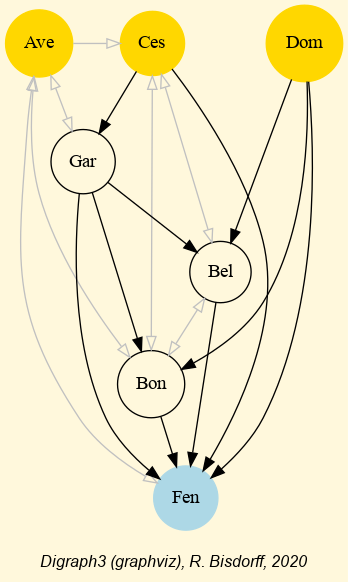
\includegraphics[width=5cm]{Figures/bestOfficeChoice.png}
\caption{Best office choice recommendation from strict outranking digraph.}
\label{fig:6.4}       % Give a unique label
\end{figure}

\section{Weakly ordering the outranking digraph}
\label{sec:6.6}

To get a more complete insight in the overall strict outranking situations, we may use the \texttt{RankingByChoosingDigraph} constructor imported from the \texttt{transitiveDigraphs} module for computing a \textbf{ranking-by-choosing} result from the codual, i.e. the strict outranking digraph instance $gcd$ (see above). If the computing node supports multiple processor cores, best and worst choosing iterations are run in parallel (see Line 3 below).

\begin{lstlisting}
>>> from transitiveDigraphs import RankingByChoosingDigraph
>>> rbc = RankingByChoosingDigraph(gcd)
 Threading ...  # multiprocessing if 2 cores are available
 Exiting computing threads
>>> rbc.showRankingByChoosing()
 Ranking by Choosing and Rejecting
    1st ranked ['D']
       2nd ranked ['C', 'G']
       2nd last ranked ['B', 'C', 'E']
    1st last ranked ['A', 'F']
>>> rbc.exportGraphViz('officeChoiceRanking')
 *---- exporting a dot file for GraphViz tools ---------*
  Exporting to officeChoiceRanking.dot
  dot -Grankdir=TB -Tpng officeChoiceRanking.dot\
                   -o officeChoiceRanking.png
\end{lstlisting}

\begin{figure}[h]
\sidecaption
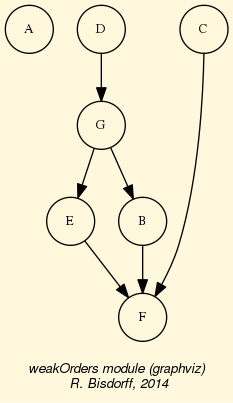
\includegraphics[width=6cm]{Figures/officeChoiceRanking.png}
\caption{In this \textbf{ranking-by-choosing} method, where we operate the \emph{epistemic fusion} of iterated (strict) best and worst choices, compromise alternative $D$ is now ranked before compromise alternative $G$. The overall partial ordering result shows again the important fact that the most expensive site $A$, and the cheapest site $C$, both appear incomparable with most of the other alternatives, as is apparent from the Hasse diagram of the ranking-by-choosing result here.} 
\label{fig:6.5}       % Give a unique label
\end{figure}
	   
The best choice recommendation appears hence depending on the very importance the CEO is attaching to each of the three decision objectives he is considering. In the setting here, where he considers that \emph{maximizing the future turnover} is the most important objective followed by \emph{minimizing the Costs} and, less important, \emph{maximizing the working conditions}, site $D$ represents actually the best compromise. However, if \emph{Costs} do not play much a role, it would be perhaps better to decide to move to the most advantageous site $A$; or if, on the contrary, \emph{Costs} do matter a lot, moving to the cheapest alternative $C$ could definitely represent a more convincing recommendation. 

\noindent \textbf{Exercise:}

\noindent It might be worth modifying these criteria significance weights in the \texttt{officeChoice.py} data file in such a way that:
\begin{itemize}
\item All criteria under an objective appear \emph{equi-significant}, and
\item All three decision objectives are considered \emph{equally important}.
\end{itemize}
What will become the best choice recommendation under this working hypothesis? \footnote{See also Lecture 7 notes from the MICS Algorithmic Decision Theory course \citep{ADT-L7}.} 


%%%%%%% The chapter bibliography
%\normallatexbib
\clearpage
%\phantomsection
%\addcontentsline{toc}{section}{Chapter Bibliography}
\bibliographystyle{spbasic}
%\typeout{}
\bibliography{03-backMatters/reference}
%\chapter{Computing a best choice recommendation}
\label{sec:6}

\abstract*{To be written.}

\abstract{To be written.}
\begin{quotation}
“... The goal of our research was to design a resolution method ... that is easy to
put into practice, that requires as few and reliable hypotheses as possible, and that
meets the needs [of the decision maker]...” -- \citep*{ROY-1966}.
\end{quotation}

\section{What site to choose ?}
\label{sec:6.1}

A SME, specialized in printing and copy services, has to move into new offices, and its CEO has gathered seven \textbf{potential office sites} (see Table \ref{tab:6.1}).

\begin{table}[h]
\caption{The potential new office sites}
\label{tab:6.1}       % Give a unique label
\begin{center}
  %\begin{small}
    \begin{tabular}{c|l|l|l}
      \svhline\noalign{\smallskip}
      ID & Name & Address & Comment\\
      \noalign{\smallskip}\hline\noalign{\smallskip}
    A &   Ave  &  Avenue de la liberté &  High standing city center\\
    B &   Bon  &  Bonnevoie &             Industrial environment\\
    C &   Ces  &  Cessange &              Residential suburb location\\
    D &   Dom  &  Dommeldange &           Industrial suburb environment\\
    E &   Bel  &  Esch-Belval &           New and ambitious urbanization far from the city\\
    F &   Fen  &  Fentange &              Out in the countryside\\
      G &   Gar  &  Avenue de la Gare &     Main city shopping street\\
      \noalign{\smallskip}\hline
    \end{tabular}
  %\end{small}
\end{center}
\end{table}

Three \textbf{decision objectives} are guiding the CEO's choice:
\begin{enumerate}
\item \emph{minimize} the yearly costs induced by the moving,
\item \emph{maximize} the future turnover of the SME,
\item \emph{maximize} the new working conditions.
\end{enumerate}

The decision consequences to take into account for evaluating the potential new office sites with respect to each of the three objectives are modelled by the following \emph{coherent family of criteria} \footnote{See \citealp{ROY-2000}}.
\begin{table}[h]
\caption{The family of performance criteria}
\label{tab:6.2}       % Give a unique label
\begin{center}
    \begin{tabular}{l|l|l|l}
      \svhline\noalign{\smallskip}
      Objective & ID & Name &  Comment\\
      \noalign{\smallskip}\hline\noalign{\smallskip}
    Yearly costs  &       C &   Costs &       Annual rent, charges, and cleaning\\
    \             &  \      & \        &  \ \\
    Future turnover   &   St &   Standing &    Image and presentation\\
    Future turnover   &   V  &  Visibility &  Circulation of potential customers \\
    Future turnover   &   Pr  & Proximity  &  Distance from town center\\
    \                 &   \   & \          &  \  \\
    Working conditions &  W  &  Space   &     Working space\\
    Working conditions &  Cf &  Comfort  &    Quality of office equipment\\
    Working conditions &  P  &  Parking  &    Available parking facilities\\
      \noalign{\smallskip}\hline
    \end{tabular}   
  \end{center}
\end{table}

The evaluation of the seven potential sites on each criterion are gathered in the following \emph{performance tableau}.
\begin{table}[h]
\caption{Performance evaluations of the potential office sites}
\label{tab:6.3}       % Give a unique label
\begin{center}
    \begin{tabular}{l|c|c|c|c|c|c|c|c}
      \svhline\noalign{\smallskip}
    Criterion  &   weight &  A  &      B &       C &       D &       E &        F &        G\\
       \noalign{\smallskip}\hline\noalign{\smallskip}

    Costs     &    45.0  &   35.0K€ &  17.8K€  & 6.7K€  &  14.1K€ &  34.8K€ &  18.6K€ &  12.0K€\\
    \      &        \    &   \      &  \     &   \     &   \    &    \    &    \    &    \ \\
    Proximity     &     32.0  &   100    &  20 &      80    &   70    &   40    &   0    &    60 \\
    Visibility     &     26.0  &   60     &  80  &     70    &   50    &   60    &   0    &    100 \\
    Standing     &     23.0  &   100   &   10   &    0     &   30    &   90    &   70   &    20 \\
    \        &      \    &   \     &   \    &    \     &   \     &   \     &   \    &    \  \\
    Working space     &     10.0  &   75    &   30   &    0     &   55    &   100   &   0    &    50  \\
    Working comfort     &      6.0  &   0     &   100  &    10    &   30    &   60    &   80   &    50 \\
    Parking     &      3.0  &   90    &   30   &    100   &   90    &   70    &   0    &    80 \\
      \noalign{\smallskip}\hline
    \end{tabular}
  \end{center}
\end{table}

All criteria, except the \emph{Costs} Criterion, admit for grading a qualitative satisfaction scale from $0\%$ (worst) to $100\%$ (best). We may thus notice in Table \ref{tab:6.3} that site 'A' is the most expensive, but also $100\%$ satisfying the \emph{Proximity} as well as the  \emph{Standing} criterion. Whereas the site 'C' is the cheapest one; providing however no satisfaction at all on both the \emph{Standing} and the \emph{Working Space} criteria.

In Table \ref{tab:6.3} we may also notice that the \emph{Costs} criterion admits the highest significance ($45.0$), followed by the \emph{Future turnover} criteria $(32.0 + 26.0 + 23.0 = 81.0)$, The \emph{Working conditions} criteria are the less significant $(10.0 + 6.0, + 3.0 = 19.0)$. It follows that the CEO considers \emph{maximizing the future turnover} the most important objective ($81.0$), followed by minizing the yearly costs ($45.0$), and less important, \emph{maximizing working conditions} ($19.0$). 

Concerning yearly costs, we suppose that the CEO is indifferent up to a performance difference of $1000.00$€, and he actually prefers a site if there is at least a positive difference of $2500.00$€. The grades observed on the six qualitative criteria (measured in percentages of satisfaction) are very subjective and rather imprecise. The CEO is hence indifferent up to a satisfaction difference of $10\%$, and he claims a significant preference when the satisfaction difference is at least of $20\%$.  Furthermore, a satisfaction difference of $80\%$ represents for him a \emph{considerably large} performance difference, triggering the case given a polarisation of the preferential situations (see \citet{BIS-2013}). 

In view of Table \ref{tab:6.3}, what is now the office site we may recommend to the CEO as \textbf{best choice}?

\section{The given performance tableau}
\label{sec:6.2}


A corresponding, \texttt{PerformanceTableau}\index{PerformanceTableau} object, saved in file \texttt{officeChoice.py} is provided in the \texttt{examples} directory of the \Digraph resources. We may inspect its actual content with the computing resources provided by the \texttt{perfTabs}\index{perfTabs} module.
\begin{lstlisting}[caption={Inspecting the \texttt{officeChoice} performance tableau},label=list:6.1]
>>> from perfTabs import PerformanceTableau
>>> t = PerformanceTableau('examples/officeChoice')
>>> t
 *------- PerformanceTableau instance description ------*
   Instance class     : PerformanceTableau
   Instance name      : officeChoice
   Actions            : 7
   Objectives         : 3
   Criteria           : 7
   NaN proportion (%) : 0.0
   Attributes         : ['name', 'actions', 'objectives',
                         'criteria', 'weightPreorder',
			 'NA', 'evaluation']
>>> t.showPerformanceTableau()
 *----  performance tableau -----*
  Criteria|  'C'        'Cf'   'P'   'Pr'   'St'   'V'    'W'   
  Weights |  45.00      6.00   3.00  32.00  23.00  26.00  10.00    
  --------|----------------------------------------------------
   'Ave'  | -35000.00   0.00  90.00 100.00 100.00  60.00  75.00  
   'Bon'  | -17800.00 100.00  30.00  20.00  10.00  80.00  30.00  
   'Ces'  |  -6700.00  10.00 100.00  80.00   0.00  70.00   0.00  
   'Dom'  | -14100.00  30.00  90.00  70.00  30.00  50.00  55.00  
   'Bel'  | -34800.00  60.00  70.00  40.00  90.00  60.00 100.00  
   'Fen'  | -18600.00  80.00   0.00   0.00  70.00   0.00   0.00  
   'Gar'  | -12000.00  50.00  80.00  60.00  20.00 100.00  50.00  
\end{lstlisting}

We thus recover all the input data. To measure the actual preference discrimination we observe on each criterion, we may use the \texttt{showCriteria()}\index{perfTabs!schowCriteria()} method.
\begin{lstlisting}[caption={Inspecting the performance criteria},label=list:6.2]
>>> t.showCriteria(IntegerWeights=True)
 *----  criteria -----*
  C 'Costs'
   Scale = (Decimal('0.00'), Decimal('50000.00'))
   Weight = 45
   Threshold ind : 1000.00 + 0.00x ;  percentile:  9.5
   Threshold pref : 2500.00 + 0.00x ; percentile: 14.3
  Cf 'Comfort'
   Scale = (Decimal('0.00'), Decimal('100.00'))
   Weight = 6
   Threshold ind : 10.00 + 0.00x ;  percentile:   9.5
   Threshold pref : 20.00 + 0.00x ; percentile:  28.6
   Threshold veto : 80.00 + 0.00x ; percentile:  90.5
    ...
\end{lstlisting}

On the \emph{Costs} criterion, $9.5\%$ of the performance differences are considered insignificant and $14.3\%$ below the preference discrimination threshold (see Listing \ref{list:6.2} lines 6-7). On the qualitative \emph{Comfort} criterion, we observe again $9.5\%$ of insignificant performance differences (line 11). Due to the imprecision in the subjective grading, we notice here $28.6\%$ of performance differences below the preference discrimination threshold (Line 12). Furthermore, $100.0 - 90.5 = 9.5\%$ of the performance differences are judged \emph{considerably large} (Line 13); $80\%$ and more of satisfaction differences triggering in fact a polarisation of the preferential situation. Same information is available for all the other criteria. 
 
A colorful comparison of all the performances is shown in Figure \ref{fig:6.1} by the \emph{heatmap}\index{perfTabs!showHTMLPerformanceHeatmap} statistics, illustrating the respective quantile class of each performance. As the set of potential alternatives is tiny, we choose here a classification into performance quintiles.

\begin{lstlisting}
>>> t.showHTMLPerformanceHeatmap(colorLevels=5,\
...                              rankingRule=None)
\end{lstlisting}
    
\begin{figure}[h]
%\sidecaption
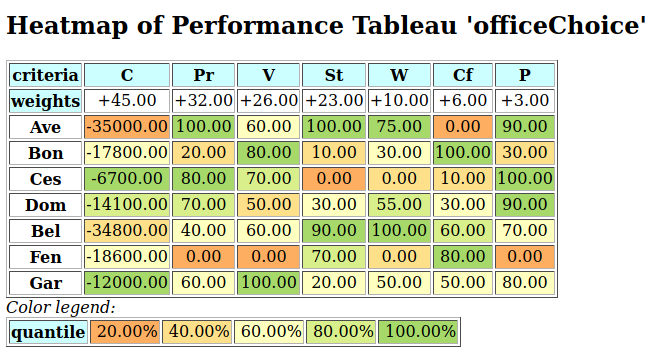
\includegraphics[width=11cm]{Figures/officeChoiceHeatmap.png}
\caption{Unranked heatmap of the office choice performance tableau.}
\label{fig:6.1}       % Give a unique label
\end{figure}

Site $Ave$ shows extreme and contradictory performances: highest \emph{Costs} and no \emph{Working Comfort} on the one hand, and total satisfaction with respect to \emph{Standing}, \emph{Proximity} and \emph{Parking facilities} on the other hand. Similar, but opposite, situation is given for site $Ces$: unsatisfactory \emph{Working Space}, no \emph{Standing} and no \emph{Working Comfort} on the one hand, and lowest \emph{Costs}, best \emph{Proximity} and \emph{Parking facilities} on the other hand. Contrary to these contradictory alternatives, we observe two appealing compromise decision alternatives: sites $Dom$ and $Gar$. Finally, site $Fen$ is clearly the less satisfactory alternative of all.

To help now the CEO choosing the best site, we are going to compute pairwise outrankings on the set of potential sites (see \citet{BIS-2013}).

\section{Computing the outranking digraph}
\label{sec:6.2}

\begin{definition}[Outranking situation]\index{outranking!situation}
For two potential office sites $x$ and $y$:
\begin{itemize}
\item $x$ \emph{outranks} $y$, denoted $(x \succsim y)$, is given when there is:
   \begin{enumerate}
     \item A \emph{majority} of criteria significance concordantly supporting that site $x$ is \emph{at least as satisfactory as} site $y$, and
     \item \emph{No considerable} counter-performance observed on any discordant criterion.      
    \end{enumerate}
\item $x$ \emph{does not outrank} $y$, denoted $(x \not\succsim y)$, is given when there is:
   \begin{enumerate}
    \item A \emph{majority} of criteria concordantly supporting that site $x$ is \emph{not at least as satisfactory as} site $y$, and
    \item \emph{No considerable} better performance observed on any discordant criterion.
    \end{enumerate}
\end{itemize}
\end{definition}
The credibility of each pairwise outranking situation\index{outranking!situation} (see \citet{BIS-2013}), denoted $r(x \succsim y)$, is measured in a bipolar significance valuation $[-1.0, 1.0]$, where \textbf{positive} terms $r(x \succsim y)\, >\, 0.0$ indicate a \textbf{validated}, and \textbf{negative} terms $r(x \succsim y)\, <\, 0.0$ indicate a \textbf{non-validated} outranking situation. The \textbf{median} value $r(x \succsim y)\, = \,0.0$ represents an \textbf{indeterminate} situation (see \citet{BIS-2004a}).   

For computing such a bipolar-valued outranking digraph from the given performance tableau $t$, we use the \texttt{BipolarOutrankingDigraph}\index{outrankingDigraphs!BipolarOutrankingDigraph} constructor from the \texttt{outrankingDigraphs}\index{outrankingDigraphs} module. The corresponding \texttt{showHTMLRelationTable}\index{digraphs!showHTMLRelationTable()} method shows here the resulting bipolar-valued adjacency matrix in a system browser window (see Fig. \ref{fig:6.2}).
\begin{lstlisting}
>>> from outrankingDigraphs import BipolarOutrankingDigraph
>>> g = BipolarOutrankingDigraph(t)
>>> g.showHTMLRelationTable()
\end{lstlisting}
\begin{figure}[h]
%\sidecaption
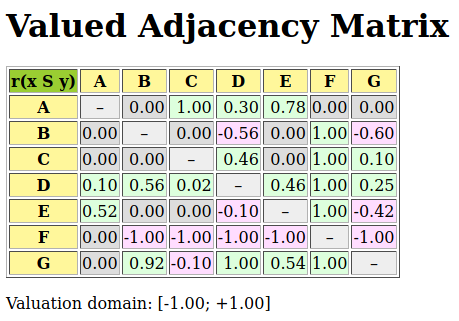
\includegraphics[width=8cm]{Figures/officeChoiceOutranking.png}
\caption{Bipolar-valued adjacency matrix.}
\label{fig:6.2}       % Give a unique label
\end{figure}
In the resulting outranking relation we may notice that Alternative 'D' is \emph{positively outranking} all other potential office sites: 'D' is a \Condorcet winner\index{Condorcet!winner}. Yet, alternatives 'A' (the most expensive) and 'C' (the cheapest) are \emph{not outranked} by any other site; they are in fact \emph{weak} \Condorcet winners.
\begin{lstlisting}
>>> g.computeCondorcetWinners()
 ['D']
>>> g.computeWeakCondorcetWinners()
 ['A', 'C', 'D']
\end{lstlisting}

We may get even more insight in the apparent outranking situations when we draw the corresponding \emph{outranking digraph}\index{outranking!digraph} (see Fig. \ref{fig:6.2}).
\begin{lstlisting}
>>> g.exportGraphViz('officeChoice')
 *---- exporting a dot file for GraphViz tools ---------*
  Exporting to officeChoice.dot
  dot -Grankdir=BT -Tpng officeChoice.dot -o officeChoice.png
\end{lstlisting}
\begin{figure}[h]
\sidecaption
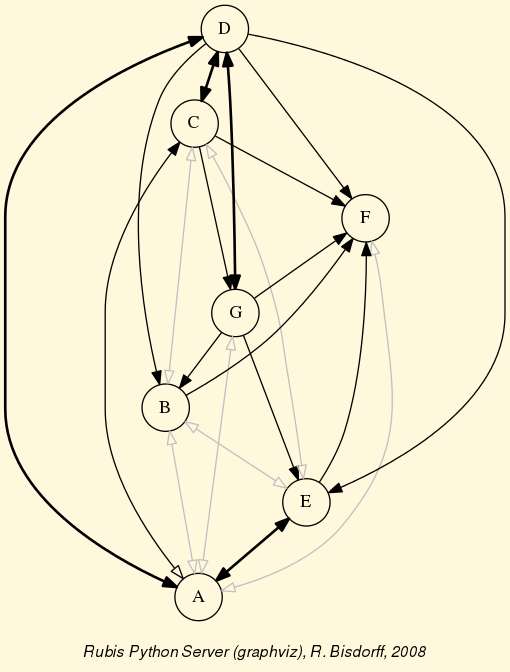
\includegraphics[width=6cm]{Figures/officeChoice.png}
\caption{The office choice outranking digraph.}
\label{fig:6.3}       % Give a unique label
\end{figure}

Outranking digraphs are \emph{weakly complete}\index{weakly complete}, i.e. for all $x$ and $y$ in $X$, $r(x \succsim y)\, <\, 0.0$ implies that $r(y \succsim x)\, \geq\, 0.0$. And, they verify the coduality principle\index{coduality principle}:  $r(x \not\succsim y) \;=\; r(y \succnsim y)$. One may furthermore check that the resulting outranking digraph $g$ here does in fact not admit any cyclic strict preference situation.

\begin{lstlisting}
>>> g.computeChordlessCircuits()
  []
>>> g.showChordlessCircuits()
  No circuits observed in this digraph.
\end{lstlisting}

\section{Computing a \Rubis best choice recommendation}
\label{sec:6.3}

Following the \Rubis outranking method\index{outranking!Rubis best choice recommendation} (see \citet{BIS-2008a}), potential best choice recommendations are determined by the outranking \emph{prekernels}\index{prekernels} --weakly independent and strictly outranking choices-- of the outranking digraph (see the tutorial on computing digraph kernels). The case given, we previously need to break open\index{digraphs!BrokenCocsDigraph} all chordless odd circuits at their weakest link.

\begin{lstlisting}
>>> from digraphs import BrokenCocsDigraph
>>> bcg = BrokenCocsDigraph(g)
>>> bcg.brokenLinks
  set()
\end{lstlisting}

As we observe indeed no such chordless circuits here, we may directly compute the \emph{prekernels} of the outranking digraph $g$.

\begin{lstlisting}[caption={Computing outranking and outranked prekernels},label=list:6.3]
>>> g.showPreKernels()
 *--- Computing preKernels ---*
    Dominant preKernels :
    ['D']
       independence :  1.0
       dominance    :  0.02
       absorbency   :  -1.0
       covering     :  1.000
    ['B', 'E', 'C']
       independence :  0.00
       dominance    :  0.10
       absorbency   :  -1.0
       covering     :  0.500
    ['A', 'G']
       independence :  0.00
       dominance    :  0.78
       absorbency   :  0.00
       covering     :  0.700
    Absorbent preKernels :
    ['F', 'A']
       independence :  0.00
       dominance    :  0.00
       absorbency   :  1.0
       covering     :  0.700
    *----- statistics -----
    graph name:  rel_officeChoice.xml
    number of solutions
     dominant kernels :  3
     absorbent kernels:  1
    cardinality frequency distributions
    cardinality     :  [0, 1, 2, 3, 4, 5, 6, 7]
    dominant kernel :  [0, 1, 1, 1, 0, 0, 0, 0]
    absorbent kernel:  [0, 0, 1, 0, 0, 0, 0, 0]
    Execution time  : 0.00018 sec.
    Results in sets: dompreKernels and abspreKernels.
\end{lstlisting}
  
We notice in Listing \ref{list:6.3} three potential best choice recommendations: the \Condorcet winner 'D' (Line 4), the triplet 'B', 'C' and 'E' (Line 9), and finally the pair 'A' and 'G' (Line 14). The best choice recommendation is now given by the \textbf{most determined} prekernel; the one supported by the most significant criteria coalition. This result is shown with the \texttt{showBestChoiceRecommendation}\index{Digraph!showBestChoiceRecommendation()} method. Notice that this method actually works by default on the broken chords digraph $bcg$.

\begin{lstlisting}[caption={Computing a best choice recommendation},label=list:6.4]
>>> g.showBestChoiceRecommendation(CoDual=False)
 *****************************************
  Rubis best choice recommendation(s) (BCR)
   (in decreasing order of determinateness)   
   Credibility domain: [-1.00,1.00]
    === >> potential best choice(s)
    * choice              : ['D']
      independence        : 1.00
      dominance           : 0.02
      absorbency          : -1.00
      covering (%)        : 100.00
      determinateness (%) : 51.03
      - most credible action(s) = { 'D': 0.02, }
    === >> potential best choice(s)
    * choice              : ['A', 'G']
      independence        : 0.00
      dominance           : 0.78
      absorbency          : 0.00
      covering (%)        : 70.00
      determinateness (%) : 50.00
      - most credible action(s) = { }
    === >> potential best choice(s)
    * choice              : ['B', 'C', 'E']
      independence        : 0.00
      dominance           : 0.10
      absorbency          : -1.00
      covering (%)        : 50.00
      determinateness (%) : 50.00
      - most credible action(s) = { }
    === >> potential worst choice(s) 
    * choice              : ['A', 'F']
      independence        : 0.00
      dominance           : 0.00
      absorbency          : 1.00
      covered (%)         : 70.00
      determinateness (%) : 50.00
      - most credible action(s) = { }
    Execution time: 0.014 seconds
\end{lstlisting}

We notice in Listing \ref{list:6.4} Line 7 above that the most significantly supported best choice recommendation is indeed the \Condorcet winner 'D' supported by a majority of $51.03\%$ of the criteria significance (see Line 12). Both other potential best choice recommendations, as well as the potential worst choice recommendation, are not positively validated as best, resp. worst choices. They may or may not be considered so. Alternative 'A', with extreme contradictory performances, appears both, in a best and a worst choice recommendation (see Lines 15 and 31) and seams hence not actually comparable to its competitors.

\section{Computing \emph{strict best} choice recommendations}
\label{sec:6.4}

When comparing now the performances of alternatives 'D' and 'G' in a pairwise perspective (see below), we notice that, with the given preference discrimination thresholds, alternative 'G' is actually \emph{certainly at least as good as} alternative 'D':  $r(G \succsim D)\, = \, +145/145\, =\, +1.0$.

\begin{lstlisting}[caption={Inspecting pairwise comparisons},label=list:6.5]
>>> g.showPairwiseComparison('G','D')
 *------------  pairwise comparison ----*
  Comparing actions : ('G', 'D')
  crit.  wght.    g(x)      g(y)    diff.  |   ind     pref    concord 	|
   =====================================================================
   'C'  45.00 -12000.00 -14100.00 +2100.00 | 1000.00 2500.00   +45.00 	| 
   'Cf'  6.00     50.00     30.00   +20.00 |   10.00   20.00    +6.00 	| 
   'P'   3.00     80.00     90.00   -10.00 |   10.00   20.00    +3.00 	| 
   'Pr' 32.00     60.00     70.00   -10.00 |   10.00   20.00   +32.00 	| 
   'St' 23.00     20.00     30.00   -10.00 |   10.00   20.00   +23.00 	| 
   'V'  26.00    100.00     50.00   +50.00 |   10.00   20.00   +26.00 	| 
   'W'  10.00     50.00     55.00    -5.00 |   10.00   20.00   +10.00 	|
   =====================================================================
    Valuation in range: -145.00 to +145.00; global concordance: +145.00
\end{lstlisting}

Yet, we must as well notice that the cheapest alternative 'C' is in fact \emph{strictly outranking} alternative 'G':  $r(C \succsim G)\, =\, +15/145\, >\, 0.0$, and $r(G \succsim C)\, =\, -15/145 \,<\, 0.0$.

\begin{lstlisting}
>>> g.showPairwiseComparison('C','G')
 *------------  pairwise comparison ----*
  Comparing actions : ('C','G')/('G','C')
  crit. wght.   g(x)     g(y)      diff.  |   ind.   pref. ('C','G')/('G','C')|
   ===========================================================================
   'C'   45.00 -6700.00 -12000.00 +5300.00 | 1000.00 2500.00    +45.00/-45.00 | 
   'Cf'   6.00    10.00     50.00   -40.00 |   10.00   20.00     -6.00/ +6.00 | 
   'P'    3.00   100.00     80.00   +20.00 |   10.00   20.00     +3.00/ -3.00 | 
   'Pr'  32.00    80.00     60.00   +20.00 |   10.00   20.00    +32.00/-32.00 | 
   'St'  23.00     0.00     20.00   -20.00 |   10.00   20.00    -23.00/+23.00 | 
   'V'   26.00    70.00    100.00   -30.00 |   10.00   20.00    -26.00/+26.00 | 
   'W'   10.00     0.00     50.00   -50.00 |   10.00   20.00    -10.00/+10.00 |
   ===========================================================================
    Valuation in range: -145.00 to +145.00; global concordance: +15.00/-15.00
\end{lstlisting}
  
To model these \emph{strict outranking} situations\index{strict outranking!situation}, we may recompute the best choice recommendation on the \textbf{codual}, the converse ($\sim$) of the dual ($-$)\footnote{Not to be confused with the dual graph of a plane graph $g$ that has a vertex for each face of $g$. Here we mean the \emph{less than} (strict converse) relation corresponding to a \emph{greater or equal} relation, or the \emph{less than or equal} relation corresponding to a (strict) \emph{better than} relation.}, of the outranking digraph instance $g$ (see \citet{BIS-2013}]), as follows:
\begin{lstlisting}[caption={Computing the strict best choice recommendation},label=list:6.6]
>>> g.showBestChoiceRecommendation(\
...                   CoDual=True,\
...                   ChoiceVector=True)   
* --- Best and worst choice recommendation(s) ---*
  (in decreasing order of determinateness)   
  Credibility domain: [-1.00,1.00]
    === >> potential best choice(s)
    * choice              : ['A', 'C', 'D']
      independence        : 0.00
      dominance           : 0.10
      absorbency          : 0.00
      covering (%)        : 41.67
      determinateness (%) : 50.59
      - characteristic vector = {
             'D': 0.02, 'G': 0.00, 'C': 0.00,
	     'A': 0.00, 'F': -0.02, 'E': -0.02, 'B': -0.02, }
    === >> potential worst choice(s) 
    * choice              : ['A', 'F']
      independence        : 0.00
      dominance           : -0.52
      absorbency          : 1.00
      covered (%)         : 50.00
      determinateness (%) : 50.00
      - characteristic vector = { 'G': 0.00, 'F': 0.00, 'E': 0.00,
	     'D': 0.00, 'C': 0.00, 'B': 0.00, 'A': 0.00, }
\end{lstlisting}				  

It is interesting to notice in Listing \ref{list:6.6} Line 9 that the \emph{strict best choice recommendation} consists in the set of weak \Condorcet winners\index{Condorcet!winner}: 'A', 'C' and 'D'. In the corresponding characteristic vector (see Lines 15-16), representing the bipolar credibility degree with which each alternative may indeed be considered a best choice (see \citet{BIS-2006a,BIS-2006b}), we find confirmed that alternative 'D' is the only positively validated one, whereas both extreme alternatives - 'A' (the most expensive) and 'C' (the cheapest) - stay in an indeterminate situation. They may be potential best choice candidates besides 'D'. Notice furthermore that compromise alternative $G$, while not actually included in any outranking prekernel, shows as well an indeterminate situation with respect to \emph{being or not being} a potential best choice candidate. 

We may also notice (see Line 16 and Line 19) that both alternatives 'A' and 'F' are reported as certainly strict outranked choices, hence as \emph{potential worst choice recommendation} . This confirms again the global incomparability status of alternative 'A' (see Fig. \ref{fig:6.3}).

\begin{lstlisting}
>>> gcd = ~(-g) # codual of g
>>> gcd.exportGraphViz(fileName='bestChoiceChoice',\
...                    bestChoice=['A','C','D'],\
...                    worstChoice=['F'])
 *---- exporting a dot file for GraphViz tools ---------*
  Exporting to bestOfficeChoice.dot
  dot -Grankdir=BT -Tpng bestOfficeChoice.dot -o bestOfficeChoice.png
\end{lstlisting}

\begin{figure}[h]
\sidecaption
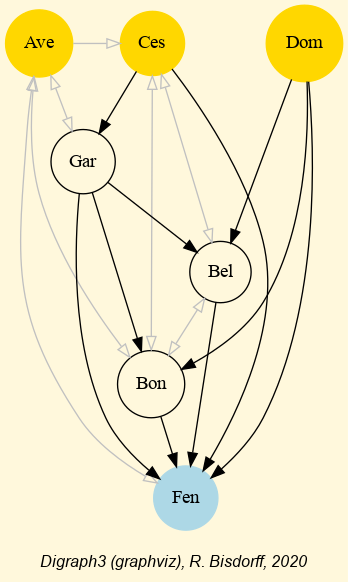
\includegraphics[width=5cm]{Figures/bestOfficeChoice.png}
\caption{Best office choice recommendation from strict outranking digraph.}
\label{fig:6.4}       % Give a unique label
\end{figure}

\section{Weakly ordering the outranking digraph}
\label{sec:6.6}

To get a more complete insight in the overall strict outranking situations, we may use the \texttt{RankingByChoosingDigraph} constructor imported from the \texttt{transitiveDigraphs} module for computing a \textbf{ranking-by-choosing} result from the codual, i.e. the strict outranking digraph instance $gcd$ (see above). If the computing node supports multiple processor cores, best and worst choosing iterations are run in parallel (see Line 3 below).

\begin{lstlisting}
>>> from transitiveDigraphs import RankingByChoosingDigraph
>>> rbc = RankingByChoosingDigraph(gcd)
 Threading ...  # multiprocessing if 2 cores are available
 Exiting computing threads
>>> rbc.showRankingByChoosing()
 Ranking by Choosing and Rejecting
    1st ranked ['D']
       2nd ranked ['C', 'G']
       2nd last ranked ['B', 'C', 'E']
    1st last ranked ['A', 'F']
>>> rbc.exportGraphViz('officeChoiceRanking')
 *---- exporting a dot file for GraphViz tools ---------*
  Exporting to officeChoiceRanking.dot
  dot -Grankdir=TB -Tpng officeChoiceRanking.dot\
                   -o officeChoiceRanking.png
\end{lstlisting}

\begin{figure}[h]
\sidecaption
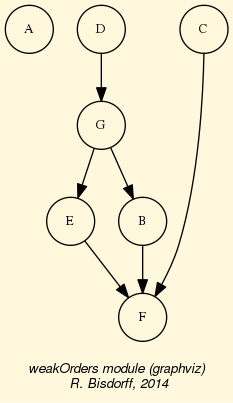
\includegraphics[width=6cm]{Figures/officeChoiceRanking.png}
\caption{In this \textbf{ranking-by-choosing} method, where we operate the \emph{epistemic fusion} of iterated (strict) best and worst choices, compromise alternative $D$ is now ranked before compromise alternative $G$. The overall partial ordering result shows again the important fact that the most expensive site $A$, and the cheapest site $C$, both appear incomparable with most of the other alternatives, as is apparent from the Hasse diagram of the ranking-by-choosing result here.} 
\label{fig:6.5}       % Give a unique label
\end{figure}
	   
The best choice recommendation appears hence depending on the very importance the CEO is attaching to each of the three decision objectives he is considering. In the setting here, where he considers that \emph{maximizing the future turnover} is the most important objective followed by \emph{minimizing the Costs} and, less important, \emph{maximizing the working conditions}, site $D$ represents actually the best compromise. However, if \emph{Costs} do not play much a role, it would be perhaps better to decide to move to the most advantageous site $A$; or if, on the contrary, \emph{Costs} do matter a lot, moving to the cheapest alternative $C$ could definitely represent a more convincing recommendation. 

\noindent \textbf{Exercise:}

\noindent It might be worth modifying these criteria significance weights in the \texttt{officeChoice.py} data file in such a way that:
\begin{itemize}
\item All criteria under an objective appear \emph{equi-significant}, and
\item All three decision objectives are considered \emph{equally important}.
\end{itemize}
What will become the best choice recommendation under this working hypothesis? \footnote{See also Lecture 7 notes from the MICS Algorithmic Decision Theory course \citep{ADT-L7}.} 


%%%%%%% The chapter bibliography
%\normallatexbib
\clearpage
%\phantomsection
%\addcontentsline{toc}{section}{Chapter Bibliography}
\bibliographystyle{spbasic}
%\typeout{}
\bibliography{03-backMatters/reference}
%\input{02-mainMatters/06-chapterBestChoice.bbl}



